\documentclass[a4paper]{report}
\usepackage{setspace}
%\usepackage{subfigure}

\pagestyle{plain}
\usepackage{amssymb,graphicx,color}
\usepackage{amsfonts}
\usepackage{latexsym}
\usepackage{amsmath}
\usepackage[a4paper, margin = 3cm, bottom = 2.5cm]{geometry}
\usepackage{algorithm}
\usepackage{algpseudocode}
\usepackage{graphicx}
\usepackage{booktabs}
\usepackage{subcaption}
\usepackage{adjustbox}
\usepackage{tikz}
\usepackage{tabularx}
\usepackage{natbib}
\usepackage{url}
\usetikzlibrary{shapes,arrows}

\newtheorem{theorem}{THEOREM}
\newtheorem{lemma}[theorem]{LEMMA}
\newtheorem{corollary}[theorem]{COROLLARY}
\newtheorem{proposition}[theorem]{PROPOSITION}
\newtheorem{remark}[theorem]{REMARK}
\newtheorem{definition}[theorem]{DEFINITION}
\newtheorem{fact}[theorem]{FACT}

\newtheorem{problem}[theorem]{PROBLEM}
\newtheorem{exercise}[theorem]{EXERCISE}
\def \set#1{\{#1\} }

\newenvironment{proof}{
PROOF:
\begin{quotation}}{
$\Box$ \end{quotation}}



\newcommand{\nats}{\mbox{\( \mathbb N \)}}
\newcommand{\rat}{\mbox{\(\mathbb Q\)}}
\newcommand{\rats}{\mbox{\(\mathbb Q\)}}
\newcommand{\reals}{\mbox{\(\mathbb R\)}}
\newcommand{\ints}{\mbox{\(\mathbb Z\)}}

\newcommand{\investigation}{investigation}

%%%%%%%%%%%%%%%%%%%%%%%%%%


\title{\vspace{-14em}\Huge Catastrophic Stock Implosion Detection}
\date{Submission date: 25/04/2024}
\author{%
    Zakariyya Tewari\thanks{%
    \textbf{Disclaimer:}
    This report is submitted as part requirement for the MY DEGREE at UCL. It is substantially the result of my own work except where explicitly indicated in the text.
    % \textit{Either:} The report may be freely copied and distributed provided the source is explicitly acknowledged.
    % \newline
    % \textit{Or:}\newline
    The report will be distributed to the internal and external examiners, but thereafter may not be copied or distributed except with permission from the author.}
    \\[1cm]
    \large Mathematical Computation\\[0.5cm]
    \large Supervisor: Prof Philip Treleaven\\[0.5cm]
    \large Technical Advisor: Dr Michal Galas
}

\begin{document}

\onehalfspacing
\maketitle

\begin{abstract}
  This thesis delves into a new category of stock market downturn known as a 'Catastrophic Stock Implosion' and develops a classification model to identify these occurrences. 
  A Catastrophic Implosion is characterized by a sudden drop in share price that persistently remains below its previous peak for an extended duration, often resulting in the stock 
  becoming a 'zombie', stagnating with minimal growth prospects.
  This research was conducted in collaboration with Banking Science and seeks to tackle the following objective:\\\\\textit{Can corporate
  fundamentals be used to predict Catastrophic Implosions effectively?}\\\\A solution to this problem holds promise for optimizing portfolio allocation strategies through the opportunity to eliminate stocks that are at risk of suffering a Catastrophic Implosion.
  The thesis comprises three experiments:
  \\\\ {\bfseries Experiment 1: Implosion Definition and Metrics.} The investigation starts with rigorously defining what a Catastrophic Implosion is and how to identify such price movements from historical data. This is crucial not only for setting the stage for the rest of the investigation, but also in addressing a significant gap in the wider literature 
  where a standardized framework for quantifying stock crashes and bankruptcy remains elusive.
  \\\\ {\bfseries Experiment 2: Methodology.} The investigation experiments with two separate approaches for detecting Catastrophic Implosions, accounting for historical data in different ways and leveraging various statistical feature engineering techniques with the objective 
  of attaining the strongest results possible.
  \\\\ {\bfseries Experiment 3: Model Evaluation.} Each approach is evaluated and refined with the goal of detecting as many implosions as possible. As part of the strategy, a concrete analysis of the key driving factors leveraged by the models is presented.
  \\\\The investigation presents the following contributions to sciences:
  \\\\1.	{\bfseries Stock implosion detection.} This investigation contributes to the scarce literature themed around stock implosions by introducing a novel definition and framework for classification via a rolling-window, Machine Learning-driven approach.
  \\\\2.	{\bfseries Analysis of key drivers behind implosions.} The investigation presents an exploration into the relationship between corporate fundamentals and Catastrophic Implosions, demystifying the nature of such price movements.
  \\\\3.	{\bfseries Effective model development for improved accuracy.} The investigation deploys novel strategies to tackle fundamental challenges such as class imbalance and hyperparameter tuning with the goal of optimizing results from an investor perspective.
\end{abstract}

\newpage

\section*{Impact Statement}
1.	{\bfseries Portfolio Management.} The model acts as a pre-screener for portfolio asset allocation, signalling in a universe of over 8000 stocks which are at risk of a Catastrophic Implosion, enhancing investment strategy by allowing for their removal.
\\\\2.	{\bfseries Factors Driving Implosions.} Through various feature selection and importance analysis techniques, the investigation discusses potential drivers behind Catastrophic Implosions from 
an array of fundamental and macroeconomic variables.
\\\\3.	{\bfseries Stock Market Forecasting.} The investigation contributes to the wider field of stock market forecasting, leveraging a range of statistical, Machine Learning and 
Deep Learning based models to predict implosions before they occur.


\tableofcontents

\listoffigures
\listoftables

\clearpage % Start a new page, optional but recommended

\setcounter{page}{1}


\chapter{Introduction}
\textit{The objective of this chapter is to provide an overview of the investigation, highlighting the motivation, research objectives, experiments carried out to meet those objectives and the contributions to science. The significance of the problem
is emphasised despite its novelty, and the chapter concludes by outlining the structure of the remaining thesis.}

\section{Motivation}
It is unsurprising that the investigation of predicting stock price movements continues to be a highly scrutinized area of research. The immense array of possible factors affecting
stock prices make modelling their movement extremely challenging. Of particular interest are stock market crashes, synonymous with financial distress. Their anomalous behaviour, yet drastic and often devastating impacts
on corporates and economies have sparked interest in analyzing the key features that could be used to forecast their occurrence. This investigation contributes to this literature by focusing on a distinct type of stock crash known as a \textit{Catastrophic Implosion}. A 
Catastrophic Implosion, in this study, is defined to be a firm-specific crash where the price of an asset falls in such a way that it is unable to recover for a significant period of time, if at all (see Figures \ref{fig:Catastrophic Stock Implosion vs Stock Crash}, \ref{fig:sample_implosions} for some examples).
The hypothesis behind such types of downturns is that they are the result of major weakness in the fundamentals of the associated company,
which increase up until investors no longer have confidence in the firm, triggering a sell-off and subsequent collapse in the stock's price. However, the novelty behind Catastrophic Implosions that distinguish them from traditional stock crash literature is that upon collapse the victim is unable to recover for an extended period of time, 
remaining at a very low market capitalization with minimal signs of possible recovery. Stocks that are currently in such a state are defined to be \textit{imploded}. While there is previous existing literature dedicated to related fields such as bankruptcy, financial distress and stock crash risk, 
there is no existing investigation, to the author's knowledge, that explores crashes described in this manner (a visualisation of the difference between the proposed Catastrophic Implosion and the typical stock crash investigated 
in previous studies can be examined in Figure \ref{fig:Catastrophic Stock Implosion vs Stock Crash}).\begin{figure}[htbp]
  \centering
  \includegraphics[width=0.9\textwidth]{acor_comparison.png}
  \caption{Stock Crash Risk vs Bankruptcy vs Catastrophic Implosion (Acorda Therapeutics)}
  \label{fig:Catastrophic Stock Implosion vs Stock Crash}
  \medskip % add some vertical space between the caption and the description
  \begin{minipage}{0.8\textwidth} % adjust the width as needed
    \small % adjust the font size as needed
    A comparison between common metrics (Stock Crash Risk and Bankruptcy) and the proposed Catastrophic Implosion.
  \end{minipage}
\end{figure} However there are several advantages to modelling these Catastrophic Stock Implosions over bankruptcy and Stock Crash Risk. While forecasting bankruptcy is of great value to investors, allowing
for the removal of predicted 'risky' stocks in their portfolio, filing for bankruptcy is not always cohesive with stock crashes. Many companies only file for bankruptcy some time after suffering crashes or do not file at all. An example is Acorda Therapeutics (shown in Figure \ref{fig:Catastrophic Stock Implosion vs Stock Crash}) - a 
pharmaceuticals company that develops medications for people with multiple sclerosis and Parkinson's disease. Acorda suffered a Catastrophic Implosion in 2021, but only announced its decision to file for Bankruptcy on 01/01/2024 (a couple of weeks ago, at the time of writing) according to pharmaceuticals newsletter provider Fierce Pharma \cite{acorda}. Had investors used a bankruptcy prediction model, 
they would have suffered the damage years ago. Thus, from 
an investor perspective, bankruptcy is not often an ideal target variable to be predicting for.\\\\On the other extreme is Stock Crash Risk, discussed further in detail in Chapter 2. Stock Crash Risk 
labels crashes based on weekly returns that deviate significantly from the yearly average. As can be observed in Figure \ref{fig:Catastrophic Stock Implosion vs Stock Crash}, there are many 'crashes' that occur prior to the bigger, final crash. In comparison 
to bankruptcy and the proposed Catastrophic Implosion, Crash Risk is very excessive.\begin{figure}[htbp]
  \centering
  \includegraphics[width=0.8\textwidth]{CHRD_crash_risk.png}
  \caption{Chord Energy Corporation (Stock Crash Risk)}
  \label{fig:crash_risk_CHRD}
  \medskip % add some vertical space between the caption and the description
  \begin{minipage}{0.8\textwidth} % adjust the width as needed
    \small % adjust the font size as needed
    Stock Crash Risk does not capture catastrophic failure.
  \end{minipage}
\end{figure} Furthermore, Figure \ref{fig:crash_risk_CHRD} illustrates an example where, despite previous 'crashes' according to Crash Risk criteria, the stock successfully \textit{explodes} in the upward direction at the end of 2020. If an investor were to hedge against or remove the stock from their portfolio, they would miss out
on this positive explosion or even suffer a loss. As a result, this investigation strives to build a hollistic metric that defines a non-recoverable, financial collapse that any investor would wish to avoid, resembling that observed in the third subfigure of Figure \ref{fig:Catastrophic Stock Implosion vs Stock Crash}. 
By detecting these unique Catastrophic Implosions, investors can choose to eliminate the corresponding securities with stronger faith that they are likely to be past a point of no return, without having to wait until bankruptcy and without severely reducing their portfolio allocations.\\\\The investigation 
approaches the challenge of classifying stock implosions primarily from a factor-based perspective. Evidence (\citep{altman1968financial}, \citep{fama1993common}, \citep{fama1992cross}) suggests 
that company fundamentals derived from balance sheet and earnings report data are versatile for bankruptcy and stock returns prediction. As a result, the investigation explores whether a similar relationship between fundamentals and implosions can also be
substantiated by developing a forecasting model equipped with such data. The hypothesis is properly defined below:\\\\\textit{Can corporate fundamentals be used to predict Catastrophic Implosions effectively?}\\\\The investigation deploys a Machine Learning driven approach to test the hypothesis, trialling a multitude of algorithms ranging from the statisical 
domain to deep learning, allowing for the modelling of non-linear interactions across a massive feature space. The data used in the investigation is provided by FactSet, in collaboration with Banking Science Limited. 

\section{Research Objectives}
In order to develop an accurate yet effective implosion prediction model that is of practical benefit to investors, several steps must be taken:
\begin{enumerate}
  \item { \bfseries Define 'Catastrophic Stock Implosion'}. First, it is imperative to clearly define the criteria for a Catastrophic Stock Implosion. Even among related literature (Crash Risk, bankruptcy) there is a lack of a wide consensus definition regarding these critical events.
  \item { \bfseries Analyse and select suitable features.} Next, an investigation into feature selection needs to be conducted. It is crucial to understand what factors can potentially lead to stock implosions and use these for the model(s).
  \item { \bfseries Develop suitable methodology.} Implementation design requires careful consideration of several factors including the amount of previous historical data used for each prediction.
  \item { \bfseries Implement model effectively.} The rarity of implosions among the wider universe of stocks examined necessitates strategies for detecting such movements and specific assessment criteria.
  \item { \bfseries Derive key factors driving implosions.} Finally post feature analysis provides invaluable insight into the factors driving corporate implosions according to the model. This opens the door to alternative, factor-based definitions for stock implosions and related events
  and provides a stronger understanding of the nature of these implosions.
\end{enumerate}

\section{Research Experiments}
This thesis outlines the full process for developing a machine-learning driven model for stock implosion classification by breaking it down into three experiments.
\\\\ { \bfseries Experiment 1 - Implosion Definition and Metrics}
\\The investigation commences with rigorously defining what it means for a stock to ‘catastrophically implode’, motivating 
the specific metrics used. An algorithm to identify such events from historical price data is constructed, and an exploratory data analysis 
of the dataset is performed, laying down the foundations for methodology design. 
\\\\ {\bfseries Experiment 2 - Methodology}
\\Within the framework of a Machine Learning, binary classification based approach, two methodologies are devised in a strive to obtain optimal 
results from an investor perspective.
\\\\ { \bfseries Experiment 3 - Model Evaluation}
\\Unique strategies for tackling class imbalance and hyperparameter tuning are developed to improve model performance across both methodologies. Following evaluation against specific classification criteria, 
an analysis into feature importance is conducted to gain valuable insights into the potential drivers behind Catastrophic Stock Implosions.

\section{Contributions to Science}
This research contributes to existing science in many ways:
\begin{enumerate}
  \item { \bfseries Stock implosion detection.} This investigation introduces a novel definition for stock crashes called Catastrophic Stock Implosions which seeks to capture catastrophic failure of a company to a greater extent than existing metrics. Several innovative feature selection, engineering and evaluation techniques scarcely applied in prior studies are 
  leveraged, resulting in a unique, Machine Learning driven classification framework and a robust model for implosion prediction.
  \item { \bfseries Analysis of key drivers behind implosions.} The investigation presents an exploration into the relationship between corporate fundamentals and implosion risk, demystifying the nature of catastrophic implosions. Over 60 fundamentals variables 
  are assessed with each model, with results suggesting potential correlations between earnings yields, earnings/assets ratios and operating expenses. Furthermore, investigations into the statistical transformations of 
  these variables are also made, providing insight into the best feature engineering techniques to employ before training.
  \item { \bfseries Effective model development for improved accuracy.} The investigation explores various strategies for enhancing the model's performance, including mitigating the class imbalance problem 
  and deploying state-of-the-art hyperparameter optimization.
\end{enumerate}
Furthermore, the investigation offers several contributions to business (investment management and trading):
\begin{enumerate}
\item {\bfseries Portfolio Management.} The model acts as a pre-screener for portfolio asset allocation, signalling stocks that are at risk of catastrophically imploding in a 
universe of over 10,000 stocks, enhancing investment strategy. The wide timeframe assessed allows for the model to be run during simulations and experimented with against different regimes.
\item {\bfseries Factors Driving Implosions.} Through feature selection and importance analysis, the investigation discusses potential drivers behind catastrophic implosions from 
an array of over 60 fundamental and macroeconomic variables.
\item {\bfseries Stock Market Forecasting.} The investigation contributes to the wider field of stock market forecasting, leveraging a range of statistical, Machine Learning and 
Deep Learning based techniques to predict implosions before they occur.
\end{enumerate}

\section{Thesis Structure}
\begin{itemize}
  \item {\bfseries Chapter 2 - Background and Literature Review.} The next chapter takes a dive into the surrounding literature including financial distress, stock crashes and bankruptcy. The distinction between implosions and these other events is emphasised, however the findings in the related studies 
  remain valuable. 
  \item {\bfseries Chapter 3 - Implosion Definition and Metrics.} The third chapter discusses possible definitions and detection methods for retrospectively identifying stock implosions from historical data, before landing on the proposed metric. An exploratory data analysis 
  based on the imploded stocks is then performed, setting the context for the methodology.
  \item {\bfseries Chapter 4 - Methodology.} The fourth chapter breaks down the challenge of modelling stock implosions in to two categories. While both solutions follow a similar, Machine Learning-driven classification framework, the stark 
  contrasts in implementation design result in models that differ in accuracy, interpretability and effectiveness.
  \item {\bfseries Chapter 5 - Model Evaluation.} The fifth chapter discusses evaluation criteria and results. Different methods are investigated to improve the model's classification ability. An analysis into the features driving the model's predictive power is conducted, and the final 
  results are discussed.
  \item {\bfseries Chapter 6 - Conclusions and Future Work.} The final chapter summarises the objectives and achievements of the investigation and points directions for further research.
\end{itemize}

\chapter{Background and Literature Review}

\textit{This chapter showcases the uniqueness of the investigation by highlighting the drawbacks of existing literature that precedes it. It starts off with introducing the domain fields, including
a brief history of factor investing and an overview of the key Machine Learning algorithms and techniques explored throughout the investigation. Finally, the related bankrutpcy prediction, financial distress 
and stock crash risk literature are discussed, affirming the uniqueness of this investigation among wider fields.}

\section{Factor-based Investing}

The investigation employs a factor-based approach to modelling catastrophic stock implosions. 'Factors' are specific characteristics that can be leveraged to explain 
asset risk and returns. Thus, factor investing is trading based on those factors that are believed to determine an asset's performance. Generally there are three broad categories of factors - fundamental, macroeconomic and 
statistical.\\\\The Capital Asset Pricing Model serves as the bedrock of factor investing. First introduced in 1962 by Jack Treynor, it describes the relationship between the expected retrurn of an asset and its risk \citep{treynor1961toward}.
The expected return is modelled as the following:
\begin{align*}
  E(r_i) &= r_f + \beta_i (E(r_m) - r_f) \\
  \\
  \text{where:} \\
  \\
  E(r_i) &= \text{Expected return of asset } i \\
  r_f &= \text{Risk-free rate of return} \\
  \beta_i &= \text{Beta of asset } i, \text{which measures its systematic risk relative to the market portfolio} \\
  E(r_m) &= \text{Expected return of the market portfolio}
\end{align*}
Hence the CAPM assumes that the expected return of an asset is entirely dependent on its beta. This results in the CAPM being quite limited in applicability. Building on this, Fama and French \citep{fama1992cross} proposed 
the following model which takes into account size and value risk factors: 
\begin{equation}
  R_{it} - R_{ft} = \alpha_{it} + \beta_1 (R_m^t - R_{ft}) + \beta_2 SMB_t + \beta_3 HML_t + \varepsilon_{it}
  \end{equation}
  
  where:
  
\begin{align*}
  R_{it} &= \text{Total return of a stock or portfolio } i \text{ at time } t \\
  R_{ft} &= \text{Risk-free rate of return at time } t \\
  R_m^t &= \text{Total market portfolio return at time } t \\
  R_{it} - R_{ft} &= \text{Expected excess return} \\
  R_m^t - R_{ft} &= \text{Excess return on the market portfolio (index)} \\
  SMB_t &= \text{Size premium (small minus big)} \\
  HML_t &= \text{Value premium (high minus low)} \\
  \beta_1, \beta_2, \beta_3 &= \text{Factor coefficients}
\end{align*}
These studies laid the foundation for a range of further studies in the field, including investigations into bankruptcy prediction \citep{altman1968financial}. Findings include 
size, value, momentum, profitability and investment as key factors that enhance factor-based strategies.


\section{Machine Learning}
Machine learning algorithms can be described as statistical methods that focus on self-improvement to make predictions. Their ability to model 
multiple features (variables) and uncover non-linear relationships, often at a large scale, pushes them far ahead of ordinary statistical methods in many applications. Given 
the multitude of possible factors to be incorporated in factor investing, they prove to be versatile in the field.\\\\There are three realms to Machine Learning - 
supervised learning, unsupervised learning and reinforcement learning. This investigation primarily focuses on supervised learning and classification. Classification is a 
fundamental task in the field of machine learning, wherein the goal is to categorize data points into predefined classes or categories based on their features. 

\subsection{Models}
The following sections give some brief introductions to the classification models employed in this investigation.

\subsubsection{Logistic Regression}
Since 1970 logistic regression has remained one of the most popular algorithms for binary classification. Logistic regression fits the logistic function to the independent variables \(x\):
\begin{equation}
  p(x) = \frac{1}{1 + e^{-x}}
\end{equation}
resulting in a probability of the sample being 1 (and 0 otherwise). The logistic function is fit by minimizing the binary cross-entropy loss: 
\begin{equation}
  l_{i} = -y_{i}\ln(p_i) - (1-y_i)\ln(1-p_i)
\end{equation}
for sample \((x_i, y_i)\). As in previous related literature, the logistic regression is used as a baseline model since it is only able to capture linear relationships.

\subsubsection{Decision Trees}
Decision trees aim to split samples into groups based on feature thresholds, with the aim of making each group as \textit{pure} as possible. The following is a high level overview of the algorithm:
\begin{enumerate}
  \item For every possible split, calculate average squared difference from the average label for each group and sum over both groups to calculate that split's loss \(l\).
  \item Pick the split that gives the lowest loss \(l*\).
  \item Repeat for each child node, and continue until stopping criteria is met.
\end{enumerate}
Decision tree methods are popular in various domains due to their low memory and computational costs.

\subsubsection{Random Forests}
Random Forests are an extension of Decision Trees designed to reduce variance through a process called Bagging. The algorithm is summarized below:
\begin{enumerate}
  \item Sample \(D_1,...,D_m\) with replacement from \(D\).
  \item For each \(D_i\) train \(h_i\) on random sample of \(k\) features.
  \item \( \hat{h} = \frac{1}{m} \sum_{i}^{m} h_i(x) \)
\end{enumerate}
By averaging the predictions over multiple decision trees, Random Forests are an example of an ensemble algorithm. By the Weak Law of Large Numbers, this average tends to the expected classifier, thus minimising variance and making 
them particularly versatile for dealing with class imbalance.

\subsubsection{Gradient Boosted Trees}
Boosting is a strategy to minimise bias. It involves adding functions ('weak learners') to a weighted ensemble. The weak learner to be added is based on minimising the loss function. There are primarily two techniques: AdaBoost and Gradient Boost.
Gradient Boosting finds the optimal weak learner by optimizing: 
\begin{equation}
  h = \text{argmin}_{\substack{h \in H}} \sum_{i=1}^{n} (h(x_i) - t_i)^2
\end{equation}
where \(t_i\) is the negative gradient of the loss function w.r.t \(H\). Then the ensemble learner is updated:
\begin{equation}
  H \leftarrow H + \alpha h
\end{equation}
XGBoost (eXtreme Gradient Boosting) is a popular open-source implementation of gradient boosting used in this investigation that incorporates regularization, among other parameters, to improve the effiency, portability and scalability of the boosting algorithm.

\subsubsection{Multilayer Perceptrons}
A Multilayer Perceptron is a complex algorithm that applies linear and non-linear functions to input data to achieve a prediction. Data is forward-propagated 
through the network, which consists of layers. Each layer has assigned to it specific weights, and at each layer the input data is transformed into a linear combination with 
its associated weights. At the end of each layer is an activation function, introducing non-linearity. After the data is passed through each layer, the final, single output 
is compared with the true value via a loss function. Similar to previous algorithms, the aim is to minimize this loss function. However, in this case the optimization is achieved 
by backpropagating the derivative of the loss function. At each layer, the weights are updated as follows: 
\begin{equation}
  W \leftarrow W - \alpha \frac{\partial L}{\partial W}
\end{equation}
Neural networks have proven superiority in several fields including time series forecasting and anomaly detection due to their ability to learn complex patterns within data. However, 
they are very prone to overfitting and difficult to interpret. In this investigation, they are trialled with all other algorithms to assess whether they provide a competitive edge in accuracy.


\subsection{Hyperparameter Tuning}
Hyperparameters resemble model configurations that are crucial for robust training. Hyperparameter tuning is the process 
of updating hyperparameters and testing models with them, with the aim of achieving optimal configurations and hence significantly improving model performance. For example, a Random Forest with 100 trees may 
work better on one specific task than a Random Forest with only 5 trees, but on another task it may perform worse. There are 
several approaches to optimizing hyperparameters, such as random search or grid search. However, this investigation takes a less-traditional path, leveraging Bayesian Optimization
to update hyperparameters during training. \\\\Bayesian Optimization works differently to Grid Search and Random Search as it uses prior evaluations 
to make future decisions. The hyperparameter space is modelled as a probability distribution, and the next hyperparameters are chosen based on an acquisition function (Expected Improvement), defined below:
\begin{equation}
  EI(x) = \int_{-\infty}^{y^*} (y^*-y) \cdot p(y | x) \, dy
\end{equation}  
In this investigation, the HyperOpt library is utilized for hyperparameter
optimization, which uses a particular version of Bayesian Optimization called Tree-based Parzen Estimation (TPE). TPE focuses on optimizing
\(p(x|y)\) where \(x\) is a given set of parameters and \(y\) is the objective value. Hence, it tries to find the best value for the objective function and selects the corresponding hyperparameters.
TPE first splits the data samples into good and bad groups based on a value \(y^*\) of the objective function:
\begin{equation}
  p(x|y) = \begin{cases}
  \text{bad if } y < y^* \\
  \text{good if } y \geq y^*
  \end{cases}
\end{equation}
  
Then the \textit{promisingness} score is calculated:
\begin{equation}
  P = \frac{p(x | good)}{p(x | bad)}
\end{equation}
This score is proportional to Expected Improvement and determines the likelihood of 
\(x\) giving a good value for the objective function. Then, by manually defining the distribution type 
for each hyperparameter (this varies depending on whether the variable is discrete vs continuous) and averaging them,
an average probability density function (PDF) can be created. This provides the probability of any \(x\) being 
\textit{good} or \textit{bad}. Hence, values that result in a high probability of being \textit{good} and low probability 
of being \textit{bad} can be chosen to maximise the promisingness score, and the process is repeated.

\subsection{Evaluation}
Evaluation is as crucial as the model training itself - assessing results requires adhering to the correct criteria while also considering the domain of the problem.

\subsubsection{Cross-Validation}
The practical value of a model comes from its ability to predict instances on unseen data. The simplest approach to mimic a real-life scenario, is to split the data so that a portion is used for training and a portion is solely kept for testing. However, during hyperparameter tuning,
one would rather perform the optimization on unseen data than on the training data. For this purpose, often an additional split in the training set is made for validation (validation set). Using the validation set,
an effective exploration into the best hyperparameters can be made while keeping the test set untouched.\\\\Cross-validation is an advancement in the train/validation split; rather 
than using just one split, the data is split into multiple sections called \textit{folds}. The model is then trained on all but one of the folds, which is used for validation, and this is repeated
for all fold combinations. This strategy improves the robustness of validation scores. However, for time series data, one must be careful about the way such folds are split. A random 
split would result in different time points scattered across different folds and models predicting the past with the future! One approach to solving this is to use a sliding window technique,
where a train-validation split is made on data at the start of the series, and then the folds move forward in time.


\subsubsection{Bias-Variance Tradeoff}
While the versatility of Machine Learning offers immense benefits, there
are also some key considerations that need to be accounted for. During evaluation, one of the crucial aspects to monitor is the bias-variance tradeoff. A model with too high of a bias leads to underfitting, failing 
to capture the underlying patterns of the data. A model with too high of a variance would lead to overfitting, where the model learns the noise of the training data and 
is unable to generalize to test data. A careful balance needs to be attained for robustness and generalization to real world scenarios. Furthermore, complex algorithms such as neural networks often suffer from the 'black box'
issue, making interpretability a challenge. This is due to the massive number of parameters and calculations that must be performed during training of these bigger models - it becomes challenging to understand 
how a given feature contributed to a particular prediction. However, the depth and complexity of these models have proven to achieve state of the art performance in a range of fields, including factor investing and algorithmic trading. Thus, 
the choice to leverage deep learning often depends on the domain context - for those that care about pure results, deep learning should be a consideration, but for those that want to understand how predictions are derived, statistical/regular 
Machine Learning algorithms may be more favourable.

\subsubsection{Metrics}
The following are commonly used metrics for assessing classification models (TP = True Positive, TN = True Negative, FP = False Positive, FN = False Negative)\\\\
\[ \text{Recall} = \frac{\text{TP}}{\text{TP} + \text{FN}} \]
Recall is the proportion of the number of positive samples correctly classified over the total number of existing positive samples. In this case, a 100\% would mean every implosion was detected.
\[ \text{Precision} = \frac{\text{TP}}{\text{TP} + \text{FP}} \]
Precision is the proportion of correctly classified positive samples over the portion of classified positive samples - it measures how well the model detects an imploded sample vs a healthy sample.
\[ \text{F1-Score} = 2 \times \frac{\text{Precision} \times \text{Recall}}{\text{Precision} + \text{Recall}} \]
F1-score is the harmonic mean of precision and recall and ranges from 0 to 1 (1 indicating perfect classification). The harmonic mean is used over a regular average to punish extreme values (e.g., a recall of 1 and
precision of 0 has F1-score 0).
\begin{align*}
  \text{Matthew's Correlation Coefficient} &= \frac{\text{TP} \times \text{TN} - \text{FP} \times \text{FN}}{\sqrt{(\text{TP} + \text{FP}) \times (\text{TP} + \text{FN}) \times (\text{TN} + \text{FP}) \times (\text{TN} + \text{FN})  }}
\end{align*}
MCC is an alternative metric that considers all possible elements of the confusion matrix. It ranges from -1 to 1, where -1 indicates a complete misclassification and 1 a perfect classification.\\\\Finally ROC (Receiver Operator Characteristic) graphs 
provide a useful visualisation of a classifier's performance, with the y-axis representing recall and x-axis representing the false positive rate. AUC represents the area under the ROC curve and is often used to quantify how well a classifier can distinguish between the 
two classes, with a higher AUC reflecting stronger ability to predict each class correctly. 

\subsubsection{Class Imbalance}
Dealing with class imbalance is a common challenge in real-world scenarios involving Machine Learning. It frequently arises when there is a skewed distribution of class labels, with one class significantly more common than the others. 
This imbalance can pose difficulties for Machine Learning models in accurately predicting instances of the minority class due to the limited data and emphasis on the majority class. This challenge is particularly relevant for this study,
where the goal is to predict implosions (the minority class) rather than the absence of implosions.
Therefore, a significant objective of this project is to address class imbalance effectively while also ensuring fairness and avoiding bias. 
Many previous studies have produced unrealistic results due to improper application of these mitigation techniques, highlighting the importance of handling class imbalance carefully and appropriately.

\subsection{Interpretability}

\subsubsection{Gini Importance}
The next sections give an overview of some of the feature importance methods leveraged in this investigation.
One of the key benefits that make Random Forests and Gradient Boosting incredibly popular for machine learning is their ability to provide context about the decisions they make 
during training and testing. For every feature, Gini Importance is calculated by averaging how much the feature decreases impurity. Impurity is calculated via the following formula:
\begin{equation}
  \sum_{y}^{C} = f_y(1-f_y)
\end{equation}
where \(C\) is number of unique labels (in this case 2) and \(f_y\) is the frequency of label \(y\) at the particular node. Impurity can 
be thought of as a measure of how 'mixed' the classes are at a given node. Hence, a feature would be deemed 'important' based on its 
ability to reduce impurity, making the groups at each tree more homogeneous. For a node \(j\), Gini importance is calculated by the following:


\begin{equation}
  ni_j = w_jC_j - w_{left(j)}C_{left(j)} - w_{right(j)}C_{right(j)}
\end{equation}
where \(ni_j\) is the importance of node \(j\), \(w_j\) is the weighted number of samples reaching node \(j\), \(C_j\) is the impurity at \(j\), \(left(j)\) represents the left child node and \(right(j)\) represents the right child node.
Finally, the feature importances for a decision tree is calculated by:
\begin{equation}
  f_i = \frac{\sum_{j: \text{node \(j\) splits on \(i\)}}ni_j}{\sum_{k \in \text{all nodes}}ni_k}
\end{equation}
where \(fi_i\) is the importance of feature \(i\). For Random Forests, the feature importances are averaged over all trees \citep{gini_importance}.

\subsubsection{SHAP Values}
Shapley values offer an alternative approach to feature importance. Derived from game theory, Shapley values assess how much each participant contributes to the outcome of the game. For a given set 
of values \(N = \{x_1, ... , x_n\}\), SHAP values can be calculated as follows:
\begin{equation}
  \phi_i(v) = \sum_{\{S \subset N\}\ \backslash\{i\}}  \frac{|S|!(n-|S|-1)!}{n!}(v(S \cup \{i\}) - v(S)) \label{eq:shap}
\end{equation}
\(\phi_i(v)\) is the marginal expected contribution of feature \(i\) - a weighted expectation of the contributions of \(i\) when 
combined with coalition \(S\) to the value \(v\) derived by the model. Note the right term of the multiplication represents the difference between 
values when feature \(i\) is included versus when it is not. The weight (left term of the sum) is defined as the probability of \(i\) making the contribution. Thus, SHAP values 
are assessing how a feature contributes to the difference \(f(x_j) - E(f(x_j))\), \(f(x_j)\) representing the prediction of \(x_j\).
SHAP values are being used increasingly 
in Machine Learning research as a way of understanding the contributions of features \citep{bluwstein2023credit}. Unlike Gini Importance, SHAP values 
can offer an indication of the direction of feature values versus target values. Furthermore, equation (\ref{eq:shap}) does not place contraints on the type of model used. The 
main drawback to SHAP values is that, as the number of features increases, the number of possible coalitions increase, hence becoming computationally expensive. However, the SHAP Python package 
offers several approximation methods to mitigate this, including KernelSHAP and TreeSHAP.\\\\It is important to realize that these techniques represent what the \textit{model} deems important based on 
its own decision-making - these cannot be used to directly confirm causal relationships between features and implosions, nor can they be used to evaluate a model's performance. However, 'important' features can be intergated into future models, and provide 
future directions for research in establishing more robust relationships.


% \subsubsection{Isolation Forest}
% While the majority of models trialled are supervised, requiring labelled data to minimize a loss function, the rarity of stock implosions probes the idea of modelling the problem as an anomaly detection problem. Unsupervised Learning has proven 
% to be quite effective for tackling such challenges, and so Isolation Forest is also experimented with. Isolation Forest is an Unsupervised Learning algorithm based off Decision Trees, with the aim of isolating anomalies with each split. The anomaly score 
% given to a data point depends on the path-length - since anomalies should be easier to separate, isolated points that are separated higher up the tree are more likely to be deemed anomalous.

\section{Related Work}
The literature relating to stock crashes and financial distress is quite complex. In many of these related fields it is clear that there remains a lack of a consensus regarding metrics used to measure implosions or crises.

\subsection{Bankruptcy Prediction and Financial Distress}
The first major breakthrough in Bankruptcy Prediction occurred in 1968 by the work of Altman \citep{altman1968financial}. He brought arise to the famous Altman Z score, which is shown below  
\begin{equation}
  \text{Z-score} = 1.2a + 1.4b + 3.3c + 0.6d + 1.0e
\end{equation}
where \(a\) represents Working Capital/Total Assets, \(b\) is Retained Earnings/Total Assets, \(c\) is EBITA/Total Assets, \(d\) is Market Value Equity/Book Value of Debt and \(e\) is Sales/Total Assets. This linear combination proved to be a very effective model, even forecasting
the collapse of many firms during the 2008 financial crisis. Despite still being used today, one small drawback noted by Altman himself was that the thresholds used at the time are now outdated.\\\\Since 1970 a range of statistical methods including multivariate discriminant analysis, logit analysis and probit analysis were tested \citep{bellovary2007review}. While
these models often displayed reasonably good performance, the re-emergence of machine learning and deep learning algorithms in 2010 motivated the use of such methods to model more complex, non-linear relationships between factors and bankruptcy. In 2017 Barboza \citep{barboza2017machine} demonstrated significant improvements to bankruptcy prediction using Machine Learning methods, 
including Random Forests and Support Vector Machines, as opposed to prior methods like the Z-score. This was despite the algorithms only incorporating 7 features. Recent studies found that AdaBoost, SVMs and logistic regression yielded strong results with more features selected based on profitability, liquidity, cash flow ratios, activity ratios and 
valutation variables. \\\\An 
important remark highlighted in many studies (\citep{bellovary2007review},\citep{shi2019overview} and \citep{zhao2024survey}) notes the range of definitions used for bankruptcy in these studies. Several studies take the event of actually filing for Chapter 7/11 bankruptcy itself. However, other measures include negative trajectory in income/cash flow \citep{mate2023comparative}, low asset/liability ratio
or signficiant drops in market value \citep{mckibben2017predicting}. The investigation by \cite{naik2021novel} identifies stock crises by observing when the 50-day moving average of a stock's price crosses below its 200-day moving average, signifying a strong downward trend.
The investigation by \cite{jiang2018corporate} even suggests multiple criteria, with only one of the following needing to be fulfilled to be deemed under 'distress': negative earnings for 2 years, net assets per share lower than face value per share, 
or abnormal financial behaviour observed by stock exchanges. Looking across all studies, each metric has its own advantages and disadvantages. For instance,
while the filing event is clear-cut in its definition, it may also lead to smaller positive samples and hence practical problems with experiments. Authors may prefer to relax criteria for a firm to qualify as 'distressed', but this would 
lead to a less-effective model. Surprisingly, definition does not tend to be a significant focal point for existing literature in the field, with often little reasoning behind the specific choice. In many cases the labels for bankruptcy are already present in the dataset and are scarcely discussed. Furthermore, there is often very little work on feature selection methods, despite the powerful impact that they could have on performance \citep{zhao2024survey}. 
One may assume from reading these studies that features are 
selected based on domain knowledge, prior studies or on a pre-existing dataset. However, as highlighted in other domains, advanced statistical, filter and wrapper feature selection techniques have shown consistency in improving model robustness.\\\\Another aspect of Machine Learning that is of particular importance to investors/corporates is model interpretability. This remains a highly-researched
field in Machine Learning, Deep Learning and AI as a whole. While in many cases authors in other domains may want to focus purely on model accuracy, investors would want to understand the decision-making behind the models they deploy. The existing studies deploying tree-based algorithms have illustrated their effectiveness of quantifying feature importance. In addition, a recent investigation \citep{bluwstein2023credit} investigating (regional) financial crises
utilizes Shapley values for post-training feature analysis, drawing relationships between credit growth and crisis risk probability.\\\\It is important
to re-emphasise the distinction between stock implosions and bankruptcy - despite the strong correlation between the two; ultimately this investigation focuses on price movement classification and not the event of bankruptcy itself. This provides an advantage to investors since it is less likely 
for a drop in stock price to occur after a firm files for bankruptcy than before. Nevertheless, the investigation's contributions are valuable in both fields. 



\subsection{Stock Crash Risk Prediction}
Stock price crash risk is another field of investigation sharing many similarities with both bankruptcy prediction and stock implosions. The notion of a stock crash comes from the idea that managers withhold
bad news regarding performance from investors, causing an accumulation of worsening conditions until it is no longer hideable - this is the point where the crash occurs. Research into measuring the risk 
of these crashes began in 2009 \citep{hutton2009opaque}. In similar respect to bankruptcy, the investigation focused on fundamental drivers, although with a stronger emphasis of the transparency of these measures.\\\\One 
key difference however is in the definition, which is much more strongly defined than current bankruptcy studies. There are a couple of steps to calculating stock crash risk. The first is to calculate
firm-specific weekly returns. The following equation:
\begin{equation}
  r_{j,s} = a_{j} + c_{1,j} r_{m,s} + c_{2,j} r_{m,s-1} + c_{3,j} r_{m,s} + c_{4,j} r_{m,s+1} + c_{5,j} r_{m,s+2} + e_{j,s}
\end{equation}
is known as the expanded market model regression. Here \(r_{j,s}\) is the weekly (normal) return of the firm \(j\) in week \(s\) and \(r_{m,s}\) is the market index return on week \(s\). Firm specific weekly returns can be calculated using this:
\begin{equation}
  w_{j,s} = \ln(1 + e_{j,s})
\end{equation} 
where \(w_{j,s}\) is the specific return for firm \(j\) in week \(s\). Using these firm-specific weekly returns, stock price crash risk can be calculated ; as detailed in \citep{habib2018stock}, there are three major metrics often used - \textit{CRASH}, \textit{NCSKEW} and \textit{DUVOL}. The first, \textit{CRASH}, is measured as follows:
\[
\textit{{CRASH}} = \begin{cases}
    1 & w_{j,s} < \mu_{y} - 3.09 \sigma_{y} \\
    0 & \text{otherwise.}
\end{cases}
\]
where \(y\) represents the current year and \(\sigma_{y}\) and \(\mu_{y}\) are the mean and standard deviation of firm-specific returns for the year \(y\) respectively. The second, \textit{NCSKEW} is calculated as follows:
\[
\textit{NCSKEW} = \frac{n}{n-1} \sqrt{\frac{\sum_{j,s} w_{3,j,s}}{\left(\frac{\sum_{j,s} w_{2,j,s}}{n-2}\right)^{3/2}}}
\]
where a higher \(\textit{NCSKEW}\) reflects stronger left-skewness in the distribution and a higher crash risk. Finally \textit{DUVOL} is calculated by: 
\[
  \textit{DUVOL}_{j,s} = \log\left(\frac{\sum_{\text{Down}} w_{2,j,s}}{(n_d - 1)\sum_{\text{Up}} w_{2,j,s}}\right)
\]
\textit{DUVOL} is the down-to-up volatility measure of crash likelihood. Returns
are grouped into 'up' weeks and 'down' weeks based on whether the returns are above or below the annual mean. Some of the key drivers of stock crash risk found resemble those for bankruptcy, such as earnings. However, other factors including 
tax avoidance, voluntary disclosure and even corporate social responsibility have been suggested to impact crash risk \citep{habib2018stock}.\\\\Interestingly, despite the overlap 
between Stock Crash Risk and Bankruptcy/Financial Distress, these topics are often studied in isolation of one another. This investigation combines aspects from both fields, with the former motivating the definition for 
a Catastrophic Implosion in Chapter 3 and the latter inspiring the classification methodology discussed in Chapter 4.


\chapter{Implosion Definition and Metrics}
\textit{In the previous chapter the lack of any concrete metrics in existing literature for quantifying stock crashes and bankruptcy was emphasised. This chapter 
proposes the novel concept of Catastrophic Stock Implosions and devises an algorithm for identifying these implosions from historical data. Following the concluded approach, an exploratory analysis of the dataset is performed, providing important
contextual considerations for methodology design.}

\section{Background}
Almost every investor connotes the notion of a 'stock crash' with a significant plunge in value of a security. However, the term itself is not a standard one - as discussed in Chapter 2 it
overlaps with 'crises', 'distress' and 'implosions', which, much in the same way, are also not robustly defined in research. Often the difference is simply in context - crises are generally
associated at a regional/economy level where distress tends to relate to specific firms. Nevertheless, whether it be a specific company on the verge of collapse or a potential economic downturn, 
predicting such events serves value to investors, corporate firms, central banks and regulatory bodies. This study introduces a new approach to modelling corporate failure by developing a classification model 
to predict significant downturns in share price that often lead to bankruptcy or removal from the exchange, and terms such events as Catastrophic Implosions. The causes behind such collapses are hypothesised
to be the result of financial weakness of companies, reflected through fundamental accounting data. Such a model 
applies particularly to an investor who seeks to refine their portfolio strategy by steering clear of stocks that are prone to suffer such disasters. As motivated in Chapter 1, there is concrete literature 
in related fields such as bankruptcy and Stock Crash Risk prediction, but neither prove ideal for capturing catastrophic failure from an investor perspective (see Figure \ref{fig:Catastrophic Stock Implosion vs Stock Crash}). Indeed, 
this chapter highlights the challenge in arriving at a robust definition for Catastrophic Implosions, and it becomes clear why there has been little research into constructing further metrics that reflect corporate failure more accurately.



\section{Dataset}
The main dataset used in this investigation was provided by FactSet in collaboration with Banking Science. All code was written on a HDFS cluster via JupyterHub, and data was extracted 
from various FactSet databases using PySpark SQL. This allowed for the distribution of processing across 12 nodes during data extraction, aggregation and model training.\\\\The FactSet database 
provides an incredible range of stocks across many exchanges globally. This investigation focuses on US equities - equities 
with their base currency as the USD. Furthermore, the stock selection is restricted to stocks traded solely on the New York Stock Exchange and Nasdaq. Stocks are extracted with historical 
data from 2000 onwards, resulting in a selection of 10,826 US stocks (although this differs to the final number used during model training/testing due to null values). Of course, many stocks do not consist of data all the way back to 2000 since they are introduced 
in later years. The distribution by industry section can be viewed in Figure \ref{fig:industry_all}. Just over a quarter of the stocks assessed are from the Financial Conglomerates industry, with 
the remaining industries roughly distributed uniformly.



\subsection{Adjusted Price}
Some data preprocessing is required before delving into possible metrics for Catastrophic Implosions. The Factset database provides raw stock prices that do not account for 
events such as splits or spin-offs. Equation \ref{eq:adjusted_price} summarizes the calculation required to adjust for these changes:

\begin{equation}\label{eq:adjusted_price}
  \text{Adjusted Price} = \text{Raw Price} \times \text{Cumulative Split Factor} \times \text{Cumulative Spinoff Factor}
\end{equation}
A split factor accounts for when a corporate splits its shares e.g., if a stock undergoes a 2-for-1 split, the factor would be 2. A spinoff factor accounts for shares distributed into a new, independent company as a result of a corporate action. 
When a company spins off a division into a separate entity, shareholders receive shares of the new company. The spinoff factor accounts for this distribution of shares. To calculate the Adjusted Price (incorporating these events), one must multiply the raw price by the 
Cumulative Split Factor and the Cumulative Spinoff Factor. The cumulative factors represent the total number of splits and spin-offs that occurred during the stock's entire timeline, ensuring that the new adjusted price accurately reflects the impact of these events on the stock's value over time. The 
data is then resampled from daily to weekly (taking the last available date per week). To ensure that the adjusted prices were calculated correctly, verifications against 
Yahoo Finance Adjusted Closing Prices were made. However, it was important to ensure that the price data and fundamentals data used in this investigation came from the same source for consistency, which is why these Yahoo Finance prices were not used instead.

\section{Implosion Definition}

\subsection{Framework}
The investigation characterizes Catastrophic Stock Implosions by breaking them down into two separate movements - one marking the start of the implosion, and one marking the 'zombie' period of decreased growth following. This framework distinguishes Catastrophic Implosions from typical metrics in related literature, 
which primarily focus only on the former. 
% This definition should be used to identify Catastrophic Implosions from historical data and label time periods appropriately, allowing for a supervised approach to model training.

% However, for Catastrophic Implosions specifically, 
% a balance between timing and value must be sought. If one chooses to quantify implosions, for instance, only after a 90\% drop in value, then there is a risk of the identification being too late - a stock may drop initially by 60\% but only reach a cumulative drop of 90\% years later, 
% potentially creating a mismatch between when the corporate fundamentals broke and when the Catastrophic Implosion occurred. On the other 
% hand, choose too light a threshold, for instance 50\%, and while the timing may be closer to the initial drop, it is more likely that the stock has not fallen low enough to be deemed on the verge of collapse. 

\subsubsection{Point of Implosion}
Deducing a suitable strategy for identifying when a Catastrophic Implosion \textit{starts} was challenging for several reasons. As discussed in Chapter 2, the range of metrics chosen for crash prediction in current literature is very diverse. Before discussing the chosen approach, it is useful to highlight the experimentation 
and methods trialled prior.\\\\The goal for defining a Catastrophic Implosion is to capture the catastrophic failure of a company through its share price. Initial approaches were inspired by literature, such as monitoring Crash Risk, identifying significant drawdowns and checking
for deviations from the moving average. By applying these methods for detecting an 'initial crash', and then checking the period after to determine if it is a sufficient 'zombie' period (see next section), Catastrophic Implosions would be identified. However, these methods all suffer from a similar issue - they all 
seek an explicit drop. It may not be apparent at first, but this study highlights that while corporate failure and stock crashes are highly correlated with one another, they are not the same. Figure (\ref{fig:cum_ret_dd_scr}) in the appendix highlights this distinction - the stock (ASTR) never suffers any \textit{significant} crash that would be 
detected by any of the prior methods, yet it is clear that it has suffered a huge loss in value over time. Furthermore, the associated company (Astra Space) as of March 2024 has gone private (off the NYSE) with the prospect of bankruptcy 'looming' according to \cite{space}. Thus, Catastrophic Implosions 
should be quantified in a way that is able to detect losses in value of all types - whether it be a sudden crash or a gradual decrease. To solve this issue, one might suggest to seek smaller drops in value, followed by the zombie period. However, this presents a danger of labelling stocks as imploded despite not actually 
suffering catastrophically (i.e., increases the risk of false positives).\\\\The proposed solution is to monitor the cumulative returns of the stock. This is the total return between two points in time one can expect by holding the asset, and is calculated as follows:
\begin{equation}\label{eq:adjusted_price}
  CR_{t_1,t_2} = \frac{{P_{t_2} - P_{t_1}}}{{P_{t_1}}}
\end{equation}
where \(P_{t_2}\) and \(P_{t_1}\) represent the adjusted price at time \(t_2\) and \(t_1\) respectively. Since cumulative returns represent the total performance of a stock at a given point in time, a significant decrease in cumulative returns reflects a decrease in the stock 
as a whole. More importantly though, a sharp drop in price is not required - instead one can check when the cumulative returns passes below a specified threshold, as shown below:
\begin{equation}
  CR_{t_0,t_i} < C, \quad 26 < i
  \label{eq:point_impl}
\end{equation}
where \(t_0\) represents the starting time of the series and \(C\) the threshold that should be specified (\(i\) starts after 26 weeks to avoid any early false alarms due to limited data). 
Thus, the approach satisfies both 'types' of implosions discussed previously, and examples for these can be viewed in the appendix (Figures \ref{fig:cum_ret_dd_scr} and \ref{fig:cum_ret_sharp}). 
The main drawback for defining the point of implosion 
in this way is that since crashes are no longer required for a Catastrophic Implosion to occur, they are sometimes missed. Indeed, when a stock does suffer from a sudden crash that satisfies the criteria for a Catastrophic Implosion, it is often the case that the point of implosion would be identified after 
the initial crash. This was one of the key advantages of using a drawdown approach, as the peaks could be recorded, thus capturing the timing of implosions more accurately. However, for this particular study, the limitation of this delay is mitigated by the methodology, since Catastrophic Implosions
are forecasted one year in advance to their occurrence. A greater emphasis is placed on the characteristics of the stocks that catastrophically implode over the timing of when an implosion occurs. If one is particular about the exact timing of an implosion, than it may be 
suitable to re-assess some of the prior methods and develop a model that works with data at a much higher frequency (e.g., monthly or weekly), although, as noted in Chapter 4, this can lead to additional challenges.

\subsubsection{Zombie Period}
While there are several possible approaches to modelling the starting point of Catastrophic Implosions, the true distinction between these market movements and regular stock crashes seen in literature is based on the period following. However, this is much easier to define, and regardless of the technique
used for detecting the point of implosion, this approach would remain the same. As a reminder, Catastrophic Implosions are implosions that cause the stock to fall in such a way that it is very unlikely to recover, signifying serious damage to the core fundamentals of the corresponding company. To observe 
how 'catastrophic' an initial crash truly was, one can observe the period following. If a stock's price rises quickly after the detected drop in cumulative returns, one can deduce that it is likely that the implosion was a result of volatility, the market as a whole 
(i.e., financial crises) or other short-term events. It is less likely that the associated corporates are suffering internally. However, if the low price is maintained for a long enough period, it is possible that significant damage on the corporate's fundamentals has been dealt. 
In quantitative terms, the following condition should be met:
\begin{equation}
  \frac{y_{\hat{t}+j} - y_{\hat{t}}}{y_{\hat{t}}} < M, \quad 0 < j < T
  \label{eq:zombie_condition}
\end{equation} Where:
\begin{align*}
& \hat{t} \text{ represents the week where the point of implosion occurred} \\
& y_{\hat{t}} \text{ represents the stock price at week } \hat{t} \\
& M \text{ is the maximum cumulative return during the 'zombie' period} \\
& T \text{ is the minimum 'zombie' period length}
\end{align*} Thus, the cumulative return should not rise higher than a specified threshold \(M\) for a given amount of time \(T\). The violation of this condition suggests the recovery of a stock, thus no longer classifying it as a Catastrophic Implosion. The parameters \(M\), \(T\) and \(C\)
are crucial to defining a Catastrophic Implosion and must be specified manually.


% \subsubsection{Proposal 1 - Stock Crash Risk}
% The first choice is to adopt 
% the Stock Crash Risk model to detect firm-specific crashes. In particular, the \textit{CRASH} model is assessed:
% \[
% \textit{{CRASH}} = \begin{cases}
%     1 & w_{j,s} < \mu_{y} - 3.09 \sigma_{y} \\
%     0 & \text{otherwise.}
% \end{cases}
% \]
% where \(w_{j,s}\) is the firm-specific weekly return of corporate \(j\) in week \(s\). By focusing on firm-specific weekly returns (discussed in detail in Chapter 2), 
% the impact of the market index, in this case the S\&P500, is eliminated, allowing for a more transparent analysis between the firm's fundamentals and implosion risk. Furthermore, prior studies 
% \citep{habib2018stock} demonstrate success in the predictability of crash risk with Machine Learning. To modify this methodology to detect catastrophic stock implosions, one can check 
% the period following the crash - if the price does not rise by a defined threshold for a given length of time, it can be hypothesised that such a crash was the result of significant
% corporate failure. Thus, this crash can be labelled as a catastrophic stock implosion. The main drawback to this approach is the requirement for an extreme drop in 
% returns - many stocks that implode do not follow this pattern, and instead drop in gradual steps or in crashes that are not extreme enough to be detected by the method.

% \subsubsection{Proposal 2 - Drawdowns}
% The second proposal is to identify 
% directional changes by the peaks of signficant drawdowns. A drawdown is defined as the movement of a stock's price from a local peak to a local trough. Thus, by identifying all major drawdowns, and checking for each whether there is 
% a rise in price within a given period afterwards, catastrophic drawdowns can be identified. The advantage of this method is that the implosion does not start when the price drops to a significant low,
% but from when the peak prior to this drop occurs. Hence, out of the three methods it proves the best at capturing the real starting points of implosions, rather than delaying it until 
% the price falls beneath a threshold. However, it shares a similar limitation to the previous approach in that it does require an explicit drop to occur.

% \subsubsection{Proposal 3 - Rolling Average}
% The third method is to assess whether there is a drop in price relative to the previous 1-year rolling average. 
% By checking whether the percentage change between the current price and rolling average price is below a specific threshold, one can then check for an implosion by checking for a rise in price afterwards (the same as prior methods). Indeed, this approach is also not dissimilar from stock crash risk literature, but by 
% utilizing the rolling average instead of the average per year, significant deviations from the trend are more likely to be captured. Furthermore, such deviations do not have to 
% occur within one week, but can instead happen over short time-spans. Hence, this technique is able to capture gradual implosions to a greater extent than the prior two techniques. The limitation of this approach is timing - by using the rolling average sharp drops will not 
% always be detected when they occur, but instead some weeks after. Furthermore, the definition requires a previous, 1-year rolling average to check for deviations from, resulting in any implosions in the first year (2000) to not be detected. \\\\(To be modified with a greater analysis and evaluation) For the rest of the investigation, the final approach, focusing on 
% deviation from rolling average, is applied. Since the experiments in Chapter 5 are conducted with yearly data, capturing the exact starting point 
% of the implosion is, for this investigation, not a crucial requirement. Thus the delay limitation of the third approach is not deemed a significant one. An example imploded stock captured by each method is illustrated in \ref{fig:Definition Comparison}.

% \begin{figure}[htbp] % 'htbp' specifies the placement preference (here: here, top, bottom, page)
%   \centering % center the figure horizontally
%   \includegraphics[width=0.8\textwidth]{3-way-comparison.png} % specify the path to your image file
%   \caption{The left figure utilizes the drawdown method. The middle figure is the rolling average and the right is 
%   the stock crash risk. The drawdown approach is able to capture the intial drop that probes the implosion, wheras 
%   the rolling average and stock crash risk approaches are delayed.} % add a caption
%   \label{fig:Definition Comparison} % add a label for referencing the figure
% \end{figure}


% \subsection{Definition 2 (Anomaly)}
% The difficulty in landing on a solid definition/labelling mechanism that captures both 'gradual' and 'sharp' implosions, while simultaneously skipping on healthy stocks is very apparent.
% As an alternative, consider the following hypothesis:\\\\ \textit{Are stock implosions distinct enough to be classified as anomalies?}\\\\If such a hypothesis proves true, then 
% the need for defining an imposion can be dropped altogether. It is important to highlight that the motivation behind detecting imploded stocks is to eliminate them from portfolios, 
% thus increasing total return. If eliminating stocks deemed as anomalous fulfills this, then the problem is solved. Indeed, the rarity of implosions both across stocks and within 
% a stock's timeline would suggest such a perspective. However, the drawback is quite evident - implosions are not the only anomalies experienced by stocks! It is possible that the (unsupervised) 
% model developed identifies anomalies that are completely unrelated to stock implosions (e.g., identifying sharp rises instead). As a result, this approach for defining implosions is treated 
% as a secondary experiment, and is only tested for imploded stock classification, not prediction.

\subsection{Definition}
To find the optimal thresholds for \(C\) (the cumulative return that the price must initially fall by), \(M\) (the maximum cumulative return that can occur during the 'zombie' period), and \(T\) (the minimum 'zombie' period length for the return to remain below \(M\)), a grid-based search strategy was conducted,
where the algorithm was run for different combinations of each parameter. The results can be seen in
Table \ref{tab:data_description} (appendix). Evident from the table, increasing the cumulative return that the stock must drop by, decreasing the threshold it should remain below after  and increasing the minimum number of weeks that the implosion should last 
all reduce the frequency of implosions, and vice versa. Of course, since the concept of Catastrophic Stock Implosions is yet to be well defined, it is difficult to judge which specific combination of thresholds should be used.
Often the best way is to verify visually. However, for this investigation an assumption was made that the number of imploded stocks should remain small, making up no more than 10\% of the entire stock selection. This is 
because Catastrophic Implosions are rare events, and too many stocks imploding would suggest failure to capture the true fundamental, catastrophic crashes that are being searched for. 
Factoring these considerations and based on consultation with the industry partners (Banking Science), the following parameters were decided on:
\begin{enumerate} 
  \item \(C = -0.8\)
  \item \(M = -0.2\)
  \item \(T = 78\)
\end{enumerate}

Thus, the final definition for a Catastrophic Implosion is as follows:\\\\
\textit{A Catastrophic Stock Implosion occurs when the cumulative return of the stock falls by at least 80\% and remains at least 20\% below the price it fell to for a minimum of 78 weeks.}
\\\\The definition provides a starting point for modelling Catastrophic Implosions, focusing exclusively on adjusted price as the main metric for quantification. However, as discussed further in Chapter 5, one of the key contributions of this 
investigation is the evaluation of driving factors behind implosions, since such factors can then be incorporated into a stronger definition. The algorithm to search and label these implosions 
can be viewed in the appendix (Figure \ref{alg:find_implosions}). An important point to emphasise here is that even when the condition 
in Eq \ref{eq:zombie_condition} is violated, the algorithm still continues its search for future implosions. However, when Eq \ref{eq:zombie_condition} is satisfied for \(T\) amount of time, the algorithm 
runs through the series until it is either violated after or the series ends (hence why \(T\) is a minimum). Also note that in the code only one implosion per stock is assumed - while there are few stocks that do implode twice, and given the newly set criteria there is nothing 
restricting a stock from doing so, the vast majority implode once. Therefore, the investigation assumes a maximum of one implosion per stock. This simplifies the modelling process in Chapter 4. 
It may seem aggressive to choose such a low \(M\), requiring the price to drop even further below \(y_{\hat{t}}\) after the initial crash. However, such 
a decision was made by process of elimination. If one were to instead try and decrease \(C\) further, this would delay the point of implosion too far from any initial crash - ideally investors 
would want to disassociate from imploding stocks as soon as possible. On the other hand, increasing \(T\) would limit the timeframe the model could be trained/tested on (e.g., using 104 weeks means that an implosion would have to remain below \(M\) for at least 2 years, 
hence no implosions would occur in 2022 as the timeframe of the dataset is 2000-2023). Thus, to ensure an appropriate proportion of stocks were considered to have imploded, the only viable remaining combination was chosen.


\section{Results}
Sample plots of Catastrophically Imploded stocks can be viewed in Figure \ref{fig:sample_implosions}. Of the 10,826 US stocks extracted, 711 suffer from at least one implosion according to the above definition (about 6.6\% of all stocks).
\begin{figure}[h] % 'h' specifies to place the figure here
  \centering
  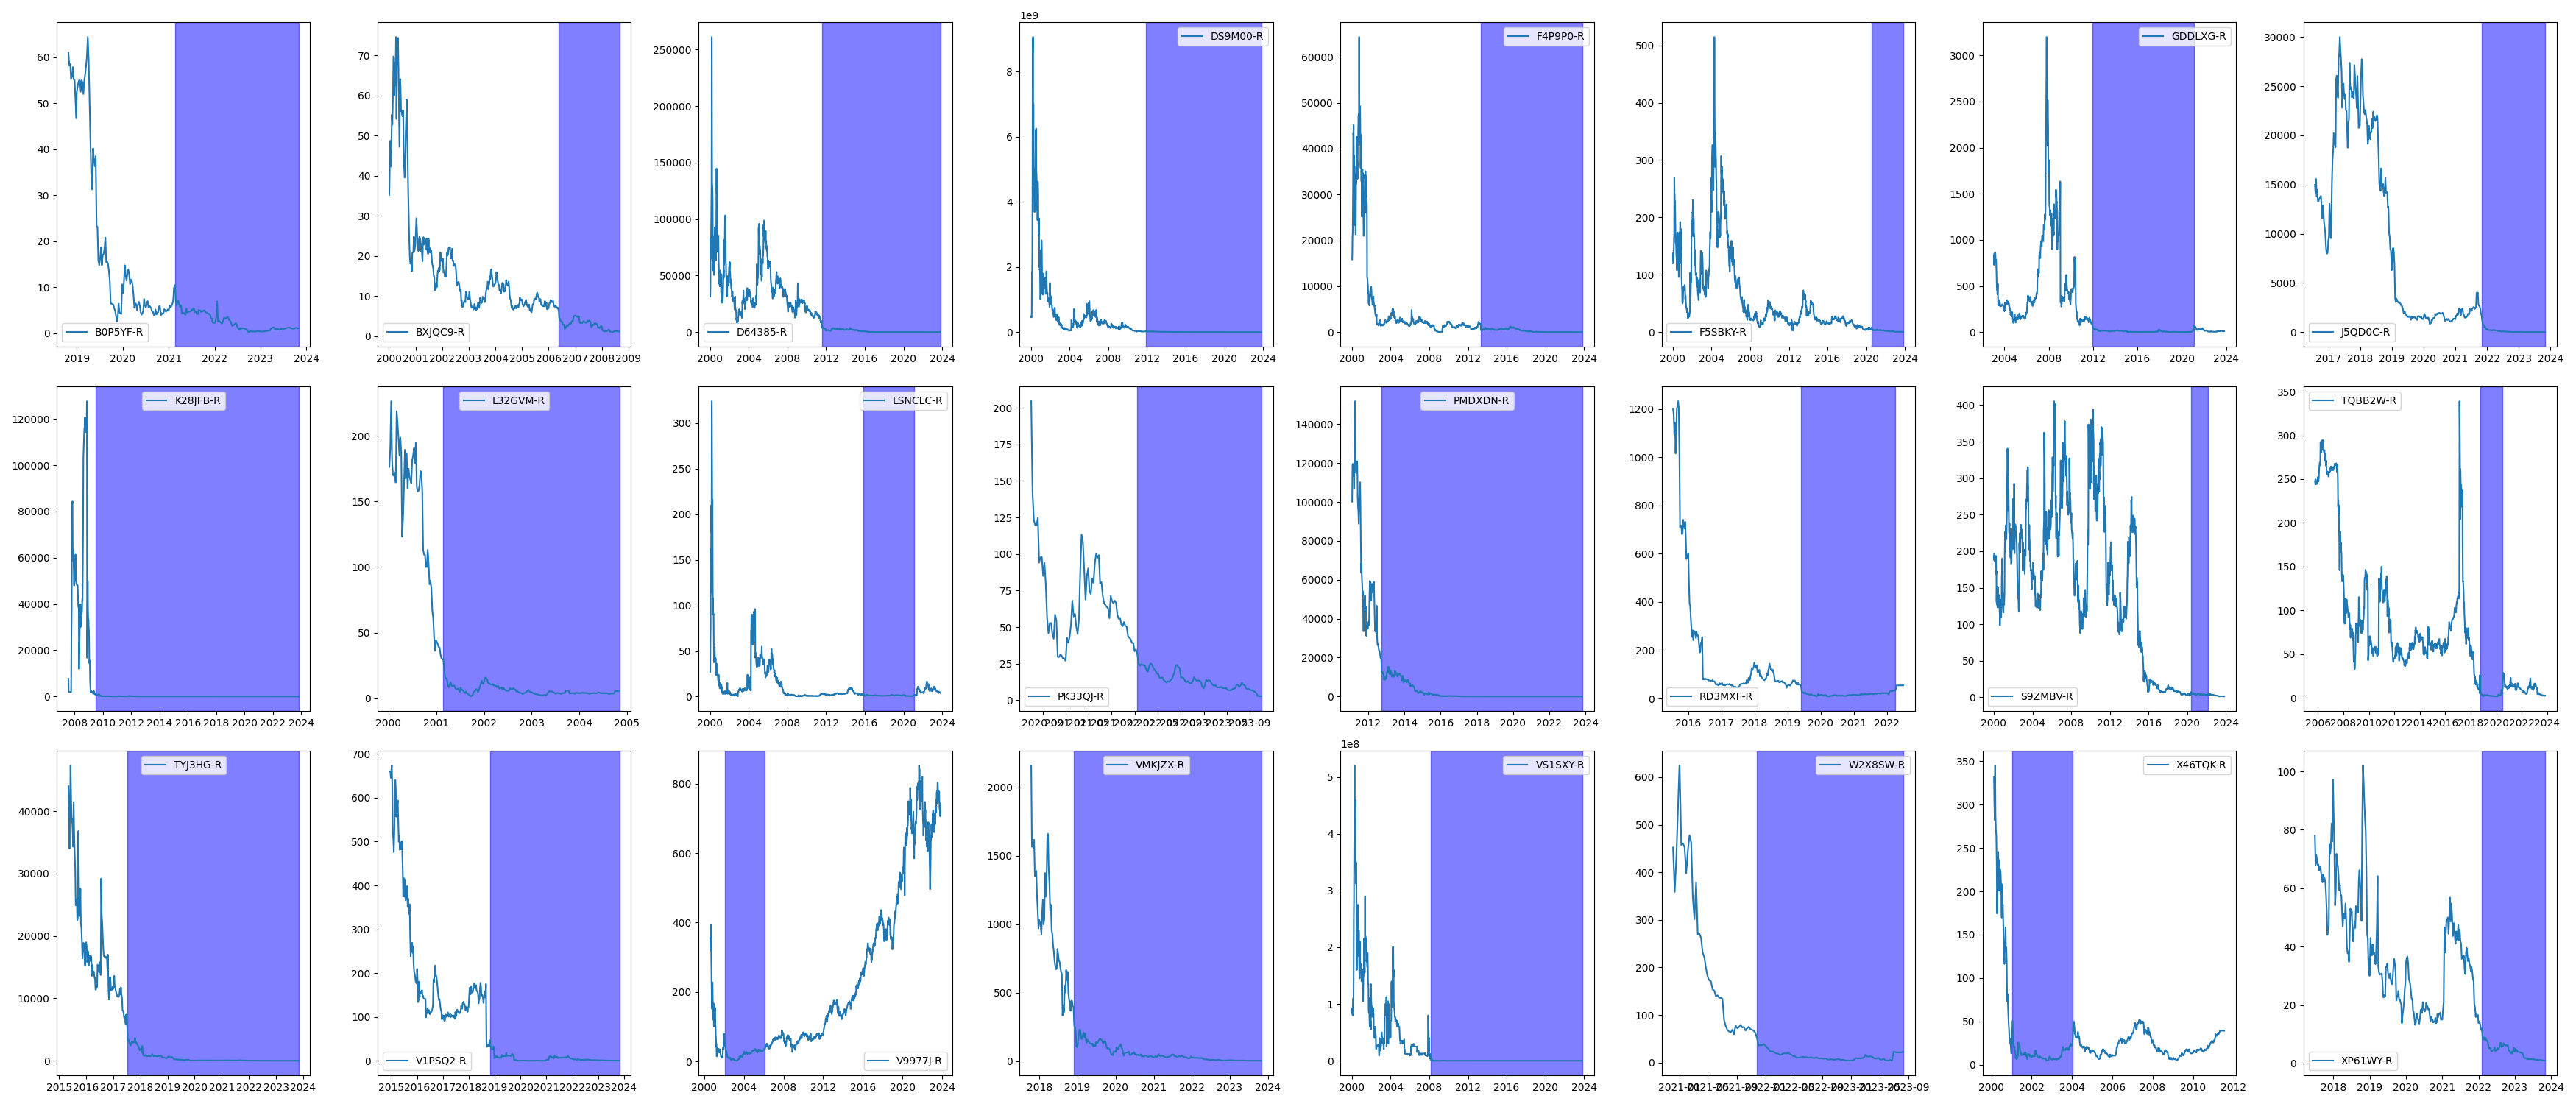
\includegraphics[width=1\textwidth]{../Stock-Implosion-Prediction-FYP/pics/sample_implosions_cum_return.png} % Replace 'image_filename' with the name of your image file
  \caption{Sample of Implosions}
  \label{fig:sample_implosions}
\end{figure} As discussed in later chapters, such a small proportion of implosions 
can lead to difficulties in prediction. Many studies choose to utilize a more flexible strategy to increase the proportion \citep{mckibben2017predicting}, but this may result in a less-effective model (this is 
another reason why, in existing literature, the definitions for stock crashes and bankruptcy are so varied). Instead, this investigation applies several techniques to tackle the class imbalance and improve the model's classification ability (see Chapter 5).
\begin{figure}[h]
  \centering
  \begin{subfigure}{0.9\textwidth}
    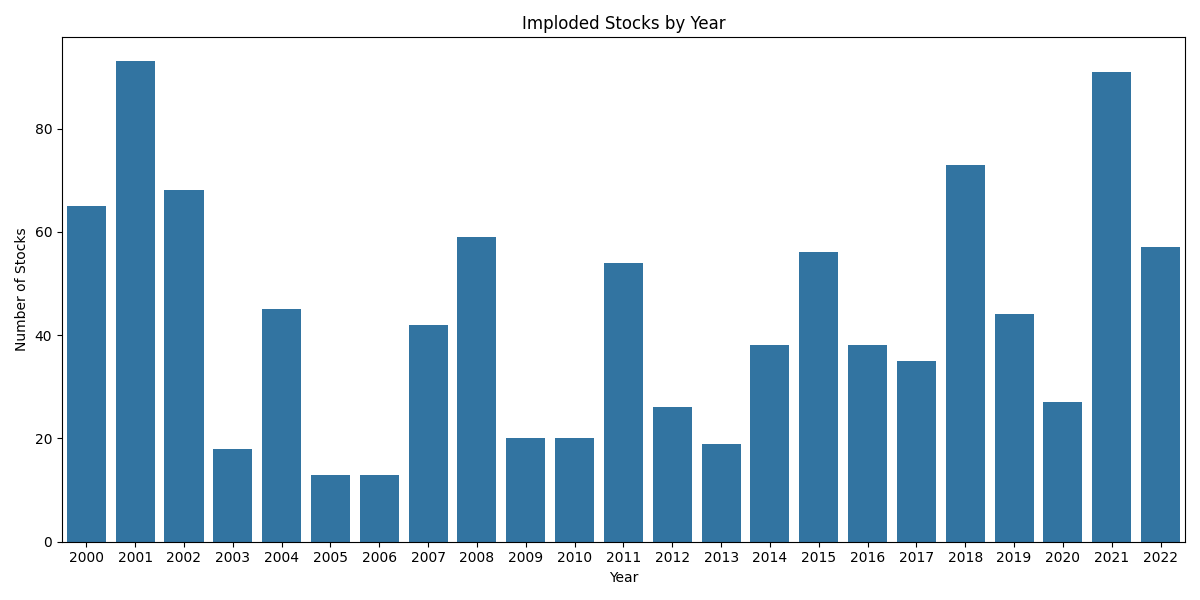
\includegraphics[width=\textwidth]{../Stock-Implosion-Prediction-FYP/pics/imploded_stocks_price.csv_per_year.png}
    \caption{Figure 1}
    \label{fig:implosions_year}
  \end{subfigure}
  \hspace{1cm}
  \begin{subfigure}{0.9\textwidth}
    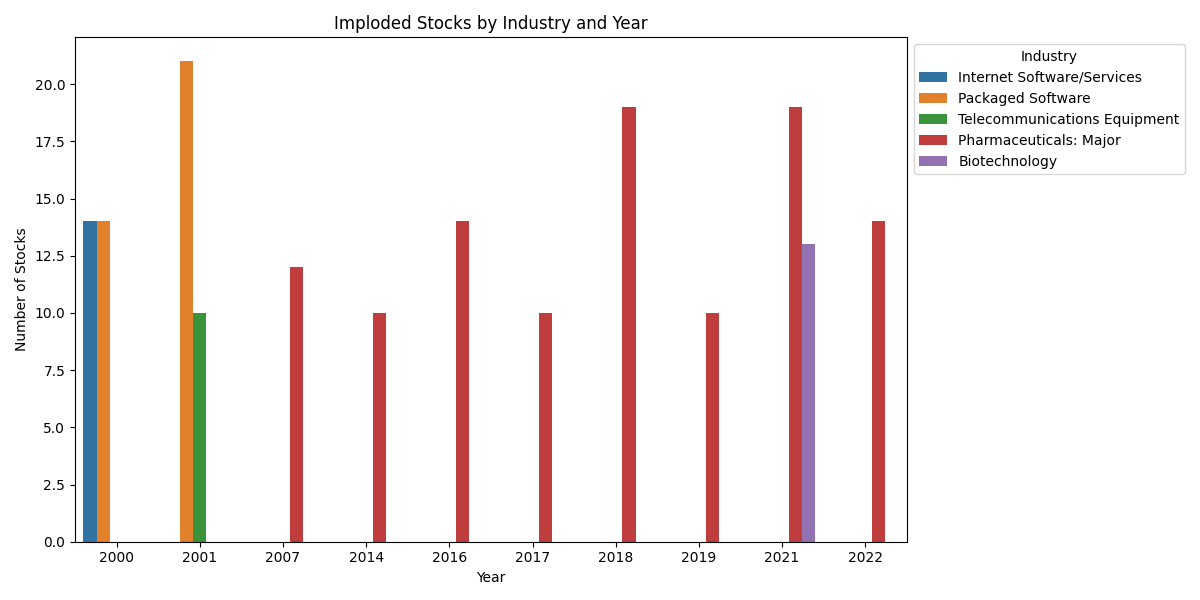
\includegraphics[width=\textwidth]{../Stock-Implosion-Prediction-FYP/pics/imploded_stocks_price.csv_by_industry.png}
    \caption{Figure 2}
    \label{fig:industry}
  \end{subfigure}
  \caption{Implosions}
  \label{fig:two_figures}
\end{figure}
\begin{figure}[h] % 'h' specifies to place the figure here
  \centering
  \begin{subfigure}{0.4\textwidth}
    \centering
    \includegraphics[width=\linewidth]{../Stock-Implosion-Prediction-FYP/pics/all_by_industry_pie.png} % Replace 'image_filename' with the name of your image file
    \caption{Stocks By Industry}
    \label{fig:industry_all}
  \end{subfigure}
  \begin{subfigure}{0.4\textwidth}
    \centering
    \includegraphics[width=\linewidth]{../Stock-Implosion-Prediction-FYP/pics/all_by_industry_implosions_pie.png} % Replace 'image_filename' with the name of your image file
    \caption{Implosions By Industry}
    \label{fig:industry_implosions_pie}
  \end{subfigure}
  \caption{Comparison of Stocks and Implosions By Industry}
  \label{fig:industry_comparison}
\end{figure}

\subsection{Examining Industry}
Figure \ref{fig:implosions_year} displays the number of implosions per year. The worst years are interestingly at opposite ends of the timeframe, being 2001 and 2021 respectively. Examining 
by industry in Figure \ref{fig:industry} provides further insight. Indeed, the implosions in Packaged Software, Internet Software/Services and Telecommunications Equipment were likely 
results from the Dot Com bubble. The following years sees the Pharmaceuticals industry consistently suffering from Catastrophic Implosions. While the factors behind this are not entirely known, 
it may be useful to dig deeper into the characteristics of some of these firms. The Pharmaceuticals industry consists of companies that develop medical drugs, and are generally deemed risky 
due to uncertainty revolving around drug development - failure to bring new drugs to the market often results in significant downturns for the company. Moreover, companies often suffer from losing exclusive rights 
to their medications. An example of this is Acorda Therapeutics (discussed in Chapter 1). \cite{acorda2} notes that the invalidation of patents protecting Acorda’s key medicines in 2017, followed by the rejection of another developmental drug, 
led to restructuring attempts and eventual bankruptcy under Chapter 11. Such timelines are sadly common in this industry. Similarly, the rise in Catastrophic Implosions
in 2021 for the Biotechnology industry is likely to be the result of a similar issue, triggered by the COVID-19 pandemic. An article by Nicholas Megaw 
highlights how vaccine firms such as Altimmune suffered devastating losses as a result of their treatments causing severe side-effects 
to patients \citep{financialtimes}.\\\\Several studies often restrict modelling to specific industries, as this would result in a dataset more specialized to the stocks 
of that industry. This investigation makes no such adjustments, examining the full spectrum of available stocks. However, industry is still considered as a feature (discussed further in Chapter 4).

\subsection{Examining Market Value}
Market value is defined by the following formula:
\begin{equation}
  \text{Market Value}_t = P_t \times \text{Number of Outstanding Shares}
\end{equation}
Market value is often used as a metric by investors for quantifying the value of a corporate, factoring in its size as well as its stock price. Thus, it is useful to inspect the market value of imploded stocks vs non-imploded stocks. Indeed, an initial analysis suggests a correlation between market capitalization and implosion likelihood. 
Figure \ref{fig:MV_Dist} highlights the distribution in market value between healthy vs imploded stocks. While 
the dataset as a whole consists of a significant proportion of small cap stocks (below \$2bn), there is a strong skewness to smaller market value for the imploded stocks. Intuitively, this makes sense - by definition corporates that catastrophically implode suffer a cumulative loss 
of over 80\% in price, hence impacting market value. In many studies, stocks with very low market value are usually neglected, since they can be quite volatile and effect predictions for larger stocks \citep{mckibben2017predicting}. However, often investors 
may want to invest in small-cap stocks, because just as there is a chance of an implosion, there is also a chance of appreciation. Therefore, the investigation chooses not to remove any small-cap stocks.
\begin{figure}[htbp] % 'htbp' specifies the placement preference (here: here, top, bottom, page)
  \centering % center the figure horizontally
  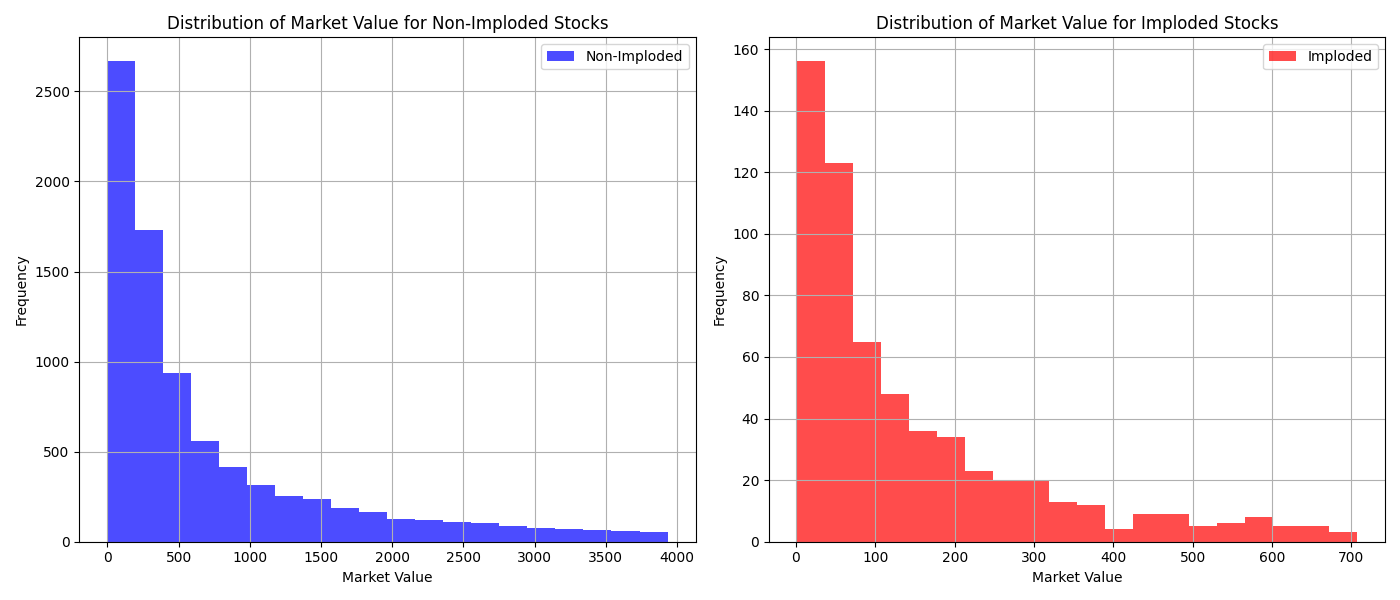
\includegraphics[width=1\textwidth]{../Stock-Implosion-Prediction-FYP/pics/market_value_distribution.png} % specify the path to your image file
  \caption{Distribution in Market Value} % add a caption
  \label{fig:MV_Dist} % add a label for referencing the figure
\end{figure}

\subsection{Examining Z-Score}
The Altman Z-Score is one of the oldest and most popular statisical models proposed for measuring bankruptcy risk. The metric is calculated as follows:
\begin{equation}
  \text{Z-score} = 1.2a + 1.4b + 3.3c + 0.6d + 1.0e
\end{equation} \label{eq:z-score}
where \(a\) represents Working Capital/Total Assets, \(b\) is Retained Earnings/Total Assets, \(c\) is EBITA/Total Assets, 
\(d\) is Market Value Equity/Book Value of Debt and \(e\) is Sales/Total Assets. While more sophisticated models today exist, with the 
ability to incorporate a much wider range of financial variables, the Altman Z-score is still often referenced as a strong baseline. Figure 
\ref{fig:Z_score} illustrates the skewness in Z-score - imploded stocks generally have a lower Z-score, indicating a higher risk of bankruptcy as opposed 
to regular stocks. This affirms the value that a prediction model for implosions would also have for bankruptcy. While the Altman Z-Score would be an excellent 
feature to include, the FactSet table unfortunately suffers from 36\% of values missing (based on the assessed dataset) and is thus not incorporated in the final model.


\begin{figure}[htbp]
  \centering
  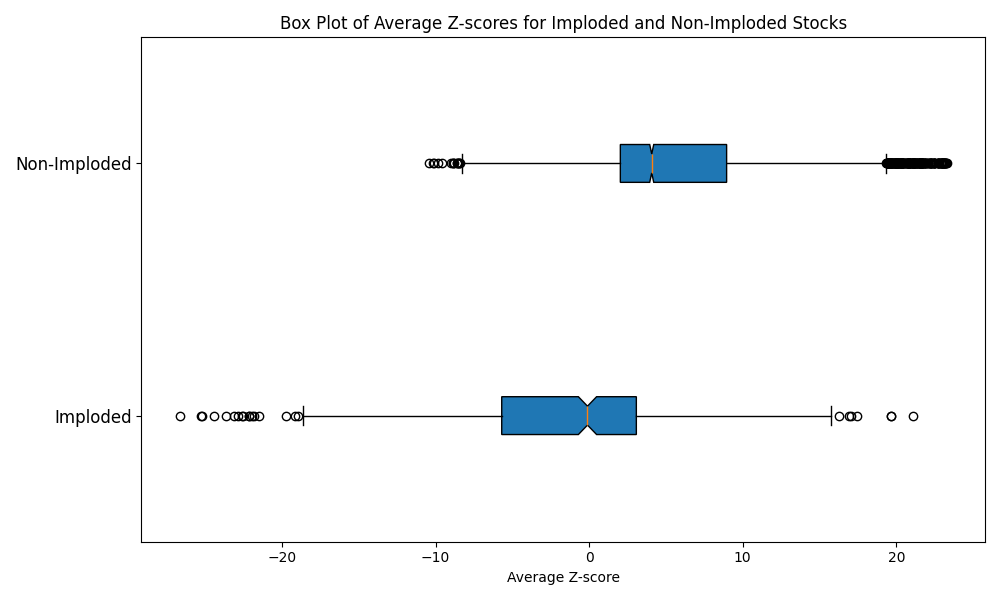
\includegraphics[width=0.6\textwidth]{../Stock-Implosion-Prediction-FYP/pics/Z_score_comparison.png} 
  \caption{Healthy Stocks Z-score vs Imploded Stocks Z-score} 
  \label{fig:Z_score} 
\end{figure}

\section{Summary}
This chapter discussed the motivation behind modelling Catastrophic Implosions as significant downturns in price that show minimal 
signs of recovery going forward, seeking to capture the essence of corporate failure more robustly compared to earlier methods found in literature. The proposed definition 
for a Catastrophic Stock Implosion is a 'crash' where the cumulative return of the stock falls by over 80\% and remains at least 20\% below the price it fell to for a minimum of 78 weeks. 
Subsequently, an exploratory data analysis of the Factset database was conducted, exploring industry, market value and previous models such as the Altman Z-score to
provide early insights into the nature of Catastrophic Implosions. The next step is to build the prediction model for detecting these Catastrophic Implosions, thereby aiding
investors in preventing significant losses within their portfolios. 


\chapter{Methodology}
\textit{The task of implosion forecasting can be approached in several ways. Key factors such as the amount of time considered for each prediction must be factored into account, and this can pave way into very 
different methodologies and model architectures. The investigation explores two lines of approach, with the first focusing on short-term historical characteristics of stocks 
and the second focusing on characteristics over a longer term.}


\section{Background}

\subsection{Initial Approaches}
The goal of this thesis was to develop a prediction model that can indicate whether a given stock at a particular point in time is at risk of Catastrophically Imploding. The problem can 
be broken down into two key subproblems - detecting \textit{which} stocks implode and, if it does, detecting \textit{when} the implosion is likely to occur. While solutions to both 
problems would hold value to investors, when handling a large portfolio of over 8000 stocks, it is reasonable to assume that an investor cares more about \textit{which} stocks are 
likely to implode, so that they can be quickly removed, rather than pinpointing when exactly they will implode. Thus, an initial strategy was to \textit{aggregate} (discussed more in final methodology) stocks over a certain time period 
and label them according to whether they implode in the subsequent time period. However, it was quickly realized that such a technique would result in a model with limited practical value to investors, as it was trained
specifically over one period to predict implosions in another period. In fact, the initial results from this model indicated strong overfitting, highlighting that the model would perform poorly when 
experimenting on unseen data. This demonstrates some of the dangers to look out for when working with time series data - it is very easy to accidentally provide a model with data it would not have access
to in a real-life application. As a research project in collaboration with Banking Science, the goal was to create a model that could not only generalize well to unseen data, but also be leveraged/adapted for backtesting 
and simulation programs. Thus, it was deemed necessary that the model be trained both across different stocks and across different time periods, solving both the \textit{which} and \textit{when} problems.

\subsection{Current Approach}
The proposed methodology aims to predict Catastrophic Implosions one year in advance of their occurrence. The following supervised methodology is applied:
\begin{equation}
  y_t = \begin{cases} 
  1 & \text{if implosion occurs in year } t+1 \\
  0 & \text{otherwise}
\end{cases}
\end{equation}
where \(t\) represents a year in time and \(y_t\) represents the target variable. Each sample
\(\mathbf{x}_t\) consists of a vector representing independent, fundamental/macroeconomic variables \(x_i\) at the current time \(t\) for a given stock. Thus, the model works across different stocks 
and different time periods, seeking to identify \textit{implosion years} before they occur. In this way, both the \textit{which} and \textit{when} subproblems are tackled. While 
this does make the underlying challenge more difficult, it also enhances the effectiveness a working model would have (e.g., one could easily apply it to data in 2024 to predict implosions in 2025). Furthermore, for backtesting and simulation
purposes, the training dataset need only be filtered to the year prior to the one being assessed for implosions. Since investors primarily care about avoiding a Catastrophic Implosion before it occurs, the years after the implosion year 
are removed from the dataset. Hence, the 'zombie' period following Catastrophic Implosions is not being forecasted. This is a sensible assumption not only because it lends well to the binary-classification approach between 'healthy' and 'catastrophic' 
years, but also because investors are unlikely to use this model on a stock that has already imploded. \\\\To predict whether a stock will suffer a Catastrophic Implosion in the subsequent year, 
previous historical data about the stock is required. However, there remains the question: \textit{How much historical data should be used per stock?} The answer 
to this question is non-trivial, and so the study conducts two separate lines of approach - one incorporating a \textit{5-year} rolling window and the other a \textit{1-year} rolling window. While 
each approach may not seem so different on the outset, there are significant contrasts in implementation that are discussed further in their respective sections. By experimenting with each approach, one can conclude 
the impact of long-term vs short-term characteristics for predicting Catastrophic Implosions.

% The task of implosion classification can be approached by various means. There is a distinction between \textit{which} types of stocks implode given their historical characteristics and 
% \textit{when} a stock implodes based on current/recent characteristics. While the ultimate objective is to build a system that can signal implosions before they occur, 
% the tradeoff between correctly classifying implosion-likely stocks versus correctly predicting when an implosion occurs needs to be carefully considered. From one perspective, 
% investors may only care that a stock is likely to implode some time in the future. Whether it is tomorrow or 5 years later, an investor would likely benefit from 
% such information (despite the ambiguity) and eliminate the stock from their selection. Such an approach would be based on the company's
% history - if there is a record of deteriorating fundamentals, there should be a higher risk of implosion. However, this would not focus on the exact timing of when an implosion would occur,
% but rather label the stock as \textit{imploding} some time in the future. From another perspective, an investor may care less about the stock's long history and want to understand what factors 
% specifically contribute to an implosion in a given year. Hence, the focus shifts to an \textit{anomaly detection} style problem, focusing on years where implosions occured and understanding 
% the fundamentals prior. With the lack of existing literature, it is difficult to assess the feasability and effectiveness 
% of each methodology. As a result, this investigation explores both lines of approach, assessing each by the following criteria:

% \begin{enumerate}
%   \item Accuracy -  how well does the approach detect implosions/imploding stocks?
%   \item Interpretability - can we understand the driving factors behind the model?
%   \item Effectiveness - how much practical value do these models bring to investors?
% \end{enumerate}
% Indeed, it is important that these criteria are carefully balanced - there is no point developing a model that has 100\% accuracy but no practical benefit to investors!

\subsection{Prerequisites}
\subsubsection{Independence}
For this methodology, the models trained for evaluation all treat each sample as \textit{independent} from the next. This differs from existing statistical models such 
as ARIMA and GARCH, as well as specific neural networks including RNNs, which factor in the previous values of samples into the next. This means that the historical data 
must be manually integrated into each sample before training takes place.

\subsubsection{Data Frequency}
The choice to work with data at a yearly frequency over a weekly/monthly frequency was deliberate. While it may be generally true that training models on more data 
can result in a stronger fit to the data, for this problem there are consequences to sampling data at a monthly frequency. The biggest drawback is the class imbalance - 
as highlighted in the Dataset Statistics sections below, both approaches suffer extreme class imbalances. Choosing a monthly 
frequency would only worsen the ratio. In addition, initial experiments with monthly data found aggregating and training to be extremely expensive computationally. Finally, as mentioned 
previously, from an investor perspective, determining \textit{which} stocks implode catastrophically was deemed more crucial than \textit{when} exactly 
it is most likely to implode, as investors would prefer to remove such stocks from their portfolios regardless of timing. Hence, choosing a yearly frequency provides a reasonable sense of time 
while keeping the focus primarily on each stock's characteristics. 

\section{Dataset}
\subsection{Background}
Before diving into the methodology design, it is imperative to understand the underlying data. This section provides a high-level overview of the primary selection of features available. As highlighted in several studies (\citep{fama1992cross}, \citep{fama1993common}, \citep{altman1968financial}), fundamental variables
have displayed state-of-the-art ability to explain cross-sectional returns and bankruptcy risk. However, literature is not clear regarding the extent of historical data to look back on for each prediction, motivating 
the exploration into assessing different-size rolling-windows.

\subsection{Fundamental Features}
The primary objective of the investigation is to leverage the fundamental factors of US corporates in an attempt to establish a relationship between them and Catastrophic Implosion risk. The FactSet database provided in association with Banking Science
offers a wealth of accounting and balance sheet variables across its universe of over 10,000 US stocks. The main variable groups include Income, Debt, Cash flow, Costs, Margins, Value and Assets. The data was pulled via SQL queries with PySpark SQL. 

\subsection{Macroeconomic Features}
While the investigation primarily investigates implosions from a factor-based perspective, the incorporation of macroeconomics serves many benefits. As highlighted previously in Figure \ref{fig:implosions_year}, 
significant numbers of implosions occur during the Dot-Com bubble and years under tightening fiscal monetary policy. While one could argue that the effects of these macroeconomic conditions would be factored 
into the fundamentals of corporates, including some features explicitly can help aid the machine learning classification, particularly the tree-based models. The following (US) macroeconomic
features were pulled from the FRED database:
\begin{enumerate}
  \item GDP - Gross Domestic Product
  \item CPI - Consumer Price Index
  \item Unemployment Rate
\end{enumerate}
The purpose of adding such variables is to provide economic context to each time window. As a result, an extensive list of macroeconomic features was not deemed necessary, especially given that many popular metrics are often highly correlated.
% GDP measures the total value of goods and services in a given year produced by a country, and is often useful for gauging a country's economic health. CPI measures the average change in price 
% of goods and services (i.e., inflation) that are consumed by people. CPI serves as a key indicator for monitoring inflation, especially for central banks. Unemployment rate measures the proportion
% of the labour force currently without a job - similar to GDP and CPI, it also provides a key indication for economic health.


\section{Approach 1 - 1-year Rolling Window}
\subsection{Background} 
The first approach focuses on predicting implosions one year in advance using previous year fundamentals only (a 1-year rolling window). The FactSet database provides an annual table of fundamental data where at a given date \(t\) the data 
represents the aggregated quarterly values between \(t-1\) and \(t\). For this approach, these values are pulled directly from the database to use in the model(s). The resulting dataframe consists of approx 100,000 rows of data, with each representing a date in time for a particular stock (at a yearly frequency).\\\\An outline of the 
remaining steps in the methodology of Approach 1 is displayed in Figure \ref{fig:approach1}.

% The first approach aims to focus on identifying \textit{imploding stocks}. In this methodology, the timing of an implosion is not a major consideration - the key focus is on the intrinsic characteristics of the stocks themselves. The aim is to analyse the historical features of a given stock 
% in an attempt to predict whether it will implode sometime in the future. The methodology focuses on identifying \textit{if} a stock will implode, instead of \textit{when} the stock implodes. The motivation for modelling the problem in this way is that it simplfies the challenge, significantly reducing 
% class imbalance (which proves to be a tricky obstacle in Approach 2). A summary of the steps involved is viewable in Figure \ref{fig:approach1}.

% \begin{figure}[h] % 'h' specifies to place the figure here
%   \centering
%   \includegraphics[width=0.9\textwidth]{approach1_method.png} % Replace 'image_filename' with the name of your image file
%   \caption{Approach 1 - Imploding Stock Prediction (Methodology)}
%   \label{fig:approach1}
% \end{figure}

% \begin{algorithm}
%   \caption{Pseudo code for SQL Data Extraction Query}
%   \begin{algorithmic}[1]
%   \State \textbf{SELECT} $t.fsym\_id$, $a.date$, $\{col\_string\}$
%   \State \textbf{FROM} $temp\_table\ t$ \textbf{INNER JOIN} 
%   \State \hspace{\algorithmicindent} (\textbf{SELECT} * \textbf{FROM} $\{table\}$
%   \State \hspace{\algorithmicindent} \textbf{LEFT JOIN} $macro\ m$ \textbf{ON} $m.year = YEAR(\{table\}.date)$
%   \State \hspace{\algorithmicindent} \textbf{WHERE} $\{table\}.date >= "2000-01-01")\ a$
%   \State \hspace{\algorithmicindent} \textbf{ON} $t.fsym\_id = a.fsym\_id$
%   \State \textbf{ORDER BY} $t.fsym\_id$, $a.date$
%   \end{algorithmic}
%   \label{fig:query}
% \end{algorithm}


\begin{figure}[h] % 'h' specifies to place the figure here
  \centering
  \includegraphics[width=0.9\textwidth]{approach1_method.png} % Replace 'image_filename' with the name of your image file
  \caption{Approach 1 - 1-year rolling window}
  \label{fig:approach1}
\end{figure}

\subsection{Feature Selection}
For this approach, feature selection is a short process, where some of the traditional steps in Machine Learning are applied to obtain a suitable set. The first step is 
to remove features that have too many null values - columns that have greater than 25\% values missing are excluded. Although some implementations of models used during experimentation 
are able to handle null values, such as XGBoost, this step was necessary to ensure consistency during evaluation with the models that cannot handle them. The next step is to create a correlation matrix 
and remove highly correlated variables, eliminating multicollinearity. Such a step introduces several benefits: removing redundancy, improved interpretability and enhanced efficiency
during model training. Finally, columns with variance lower than \(0.1\) are also removed, as these are unlikely to provide 
significant information to distinguish between the two classes. By the end, 66 features remain. Null values were imputed via forward-filling and then median-filling. Any 
null values remaining were dropped from the dataframe.\\\\Figure \ref{fig:industry} suggests that implosions can be characterized by industry, with the Pharmaceuticals and Medical industries particularly risk-prone. Hence, 
integrating this insight into the feature set is warranted. Given that industry represents a categorical variable, it is encoded using one-hot encoding, generating columns for each distinct industry where
a stock is marked as 1 if it belongs to a particular industry and 0 otherwise. This step was carried out last as the previous feature selection techniques 
should not be applied to the industry feature. However, to avoid the incorporation of too many additional features, only the largest 10 industries are encoded.

\subsection{Dataset Statistics}
A train/test split was made on the date '2020-01-01', resulting in an approximate 80/20 ratio. The following table provides an overview of the final datasets before training:
\begin{table}[htbp]
  \centering
  \begin{tabular}{|c|c|}
  \hline
  \textbf{Statistic} & \textbf{Value} \\
  \hline
  Rows of Data & 49,997 \\
  Number of Implosions & 434 \\
  Timespan & 2000-01-01 - 2020-01-01\\
  \hline
  \end{tabular}
  \caption{Train Set (Approach 1)}
  \label{tab:train_set_app1}
\end{table}

\begin{table}[htbp]
  \centering
  \begin{tabular}{|c|c|}
  \hline
  \textbf{Statistic} & \textbf{Value} \\
  \hline
  Rows of Data & 12,799 \\
  Number of Implosions & 127 \\
  Timespan & 2020-01-01 - 2023-11-02 \\
  \hline
  \end{tabular}
  \caption{Test Set (Approach 1)}
  \label{tab:test_set_app1}
\end{table}The class imbalance across the entire dataset is very sharp, with only 1\% of years classifying as implosion-years. One may notice that despite initial claims that 
the dataset consisted of approx 100,000 rows of data, the final training set includes just under 50,000 instances. In this approach, where null values could not be imputed (the entire series for 
a particular stock was unavailable), the year for that stock was dropped from the training set. However, this was not applied for the test set - where instead remaining null values were imputed 
based on the median of that year. This was necessary to keep the proportion of Catastrophic Implosions in the test set the same, ensuring a realistic scenario for testing. Such restrictions 
are not required for the training set, as this is what is used to build the model, and there is no need to apply a model to data it has been trained on!

\section{Approach 2 - 5-year Rolling Window}
\subsection{Background}
There are several limitations to Approach 1, the most notable being the small 1-year window used for prediction for each sample. While this simplifies implementation design, 
requiring few preprocessing and feature selection steps before model training, the amount of information incorporated into each sample is very limited. It is difficult to gauge 
exactly the best window size, as this is influenced by factors such as data frequency, prediction horizon and particular models trained. Thus, the best way of tackling this problem 
is experimentation. As discussed in Chapter 5, results from Approach 1 were fairly weak, with MCC scores failing to pass a threshold of 0.15. This prompted the exploration 
into alternative approaches that could incorporate more historical data for each prediction. This also aligns well with bankruptcy 
prediction theory - companies that eventually collapse often experience negative trends in growth and stability, potentially over several years.\\\\Previous studies 
often incorporate further historical information per sample via lagged features, where from a given time series, another series shifted down by \(n\) rows is created, \(n\)
representing the lookback period. However, early experiments during this investigation found that applying lagged values was problematic for several reasons. The main issue is 
that each lagged feature will introduce a null value, and since lags need to be applied separately for each stock, a single lag would introduce several thousand additional null values
that must be handled somehow. To avoid this problem while still incorporating a longer period of time, a different route was taken - aggregation. By performing multiple statistical 
aggregations over a period of time, a new feature set can be built representative of that time period. The details of the process are discussed further below.

\begin{figure}[h] % 'h' specifies to pla ce the figure here
  \centering
  \includegraphics[width=0.9\textwidth]{approach2.png} % Replace 'image_filename' with the name of your image file
  \caption{Approach 2 - 5-year rolling window}
  \label{fig:approach2}
\end{figure}

\subsection{Feature Selection}
As part of the objective to incorporate a larger rolling-window per sample for prediction, this approach addresses a signficiant gap in financial distress and 
bankruptcy prediction literature. As noted by \cite{zhao2024survey} in his literature survey of the field, feature selection remains an unexplored domain despite 
its importance in Machine Learning methodology. This approach seeks to contribute to this field by introducing a novel framework for feature selection and engineering.
% \begin{figure}[h] 
%   \centering
%   \includegraphics[width=1\textwidth]{featureselection.png}
%   \caption{Feature Selection Process}
%   \label{fig:feat_select}
% \end{figure}\\\\
The initial steps are the same as those for Approach 1 - the same query is used to pull yearly data from the FactSet database. Features 
with over 25\% null values are removed, and highly correlated/low variance variables are dropped. After this step, there are, as before, approximately 66 remaining features.
While this is not a large amount relative to the number of data points, as discussed further below,
one of the novelties of this approach comes with feature extraction. Feature extraction is the process of engineering features to create new ones that unveil hidden patterns 
within the raw data. In this case, feature extraction is used to aggregated features over the 5-year rolling window. The specific tool used generates around 20 additional aggregated features 
for every raw feature encountered, hence significantly expanding the feature space. To reduce computational costs and the possibility of overfitting, the current 
selection of features should be narrowed as much as possible before aggregation. To achieve this, the Boruta algorithm is employed.

\subsubsection{Boruta}
The Boruta algorithm is a distinct feature selection algorithm that works in conjunction with impurity-based ML models such as Decision Trees, Random Forests and Gradient Boosted Trees. The 
general steps are outlined below (\cite{boruta}):
\begin{enumerate}
  \item Randomly shuffle existing features to create new 'shadow' features and join these to the original dataset.
  \item Train the model, calculate feature importance and record all normal features that have higher importance than the strongest shadow feature.
  \item Repeat steps 1-2 for 100 iterations.
  \item Verify which features should be kept according to a binomial distribution.
\end{enumerate}It 
is important to emphasise that Boruta is (necessarily) applied \textit{before} the stocks are aggregated. This means that the dataset consists of samples where each row represents a 1-year window of data for a particular stock,
mirroring Approach 1. Hence, the data seen by Boruta is different from the data seen by the models during training. For this study, this does not pose a problem - 
Boruta is leveraged less as a way of identifying specific driving features of implosions and more to remove redundant features, narrowing the set down before aggregation. The 
validity of using Boruta for this purpose was also confirmed when repeating the experiment without applying the algorithm - results were slightly lower despite 
the much larger feature space, confirming the redundancy of many of features that would otherwise be eliminated by Boruta.\\\\Boruta 
is unable to handle null values, thus imputation is required. Forward filling is applied followed by median filling (of course, this must be done separately for each stock). The specific 
model used for Boruta was XGBoost due to its efficient run-time. Features ranked lower than 10 are retained and any higher are discarded, leaving 28 features for feature extraction.

\subsubsection{Time Series Feature Extraction}
The current dataset so far is still very similar to that of Approach 1, albeit with a smaller feature space. To incorporate a 5-year rolling window, the features are 
aggregated on a rolling-basis using an open-source library called TSFEL (Time Series Feature Extraction Library) \citep{barandas2020tsfel}. TSFEL is an efficient feature extraction library 
that applies multiple statistical, temporal and spectral transformations specific to time series features.
Statistical features include metrics such as mean, variance and percentiles, temporal features focus on patterns associated with time, such as autocorrelation and seasonality, and spectral features 
look at the frequency domain characteristics of time series, with metrics such as the Fourier transform or wavelet transform. TSFEL is very useful for applying these transformations 
(in total over 100) at a large scale. For this case, by looping through each 
stock's time series, and applying the extraction over a rolling, 5-year window, multiple aggregated features can be derived for each stock in place of the original features. The selection of a 
5-year window was made to encompass longer-term historical data while not restricting the stock selection significantly (stocks with less than 5 years worth of data cannot be assessed).\\\\Including 
the full spectrum of possible transformations results in over 1000 features. Such a large feature space is very computationally expensive to train with (and can also lead to overfitting). Thus, to narrow 
down the selection of variables, only specific transformations should be chosen from the options provided by TSFEL. These transformations are deduced based on the 
feature importances derived from initial experiments (discussed further in Chapter 5), where transformations that resulted in the highest Gini importance/SHAP values were retained. The final framework applies the transformations displayed in Figure \ref{tab:tsfel}.
\begin{table}[htbp]
  \centering
  \begin{tabular}{|c|c|}
  \hline
  \textbf{Statistical} & \textbf{Temporal} \\
  \hline
  Absolute Energy & Area Under Curve \\
  ECDF Percentile Count & Autocorrelation \\
  Entropy & Mean Absolute Diff \\
  Histogram & Median Absolute Diff \\
  Max & Mean Diff \\
  Mean & Median Diff \\
  Median & Negative Turning Points \\
  Median Absolute Deviation & Positive Turning Points \\
  Min & Sum Absolute Diff \\
  Root Mean Square &  \\
  Stdev &  \\
  Variance & \\

  \hline
  \end{tabular}
  \caption{Chosen TSFEL transformations}
  \label{tab:tsfel}
\end{table}Finally, highly correlated/low variance features are dropped and, just like in Approach 1, the industry features are concatenated on after the feature selection/extraction stages via one-hot encoding. Another 
key advantage for aggregating features in this way is that null values are much rarer, requiring very little imputation or removal from both the training and testing set. This leads to a (perhaps surprisingly) larger 
training dataset than that of Approach 1.

\subsection{Dataset Statistics}
The final train/test split was made on the date '2019-01-01' to ensure an 80/20 ratio for consistency with Approach 1. The following table provides an overview of the final datasets before training:
\begin{table}[htbp]
  \centering
  \begin{tabular}{|c|c|}
  \hline
  \textbf{Statistic} & \textbf{Value} \\
  \hline
  Rows of Data & 55,698 \\
  Number of Implosions & 308 \\
  Timespan & 2000-01-01 - 2019-01-01\\
  \hline
  \end{tabular}
  \caption{Train Set (Approach 2)}
  \label{tab:train_set_app2}
\end{table}

\begin{table}[htbp]
  \centering
  \begin{tabular}{|c|c|}
  \hline
  \textbf{Statistic} & \textbf{Value} \\
  \hline
  Rows of Data & 12,637 \\
  Number of Implosions & 114 \\
  Timespan & 2019-01-01 - 2023-11-02 \\
  \hline
  \end{tabular}
  \caption{Test Set (Approach 2)}
  \label{tab:test_set_app2}
\end{table}
The class imbalance is also the same as that of Approach 1 (1\% belonging to the implosion class).

\section{Training} 
For both methodologies, the following supervised models are trialled:
\begin{enumerate}
  \item Logistic Regression
  \item Random Forest
  \item Gradient Boosted Trees
  \item Multilayer Perceptron
\end{enumerate}
Random Forests and Gradient Boosted Trees are ensemble models, combining multiple trees to make predictions. This means they are generally adept for handling 
class imbalance (discussed further in Chapter 5). Logistic Regression is used as a baseline and is not expected to perform as effectively, and the Multilayer Perceptron 
is experimented to assess whether there are any deeper, non-linear feature interactions that could not be detected by the others. For the latter, scaling 
is applied to avoid the blow-up of model weights: 
\begin{equation}
  z = \frac{x - \mu}{\sigma}
\end{equation}
where \(z\) represents the scaled value.

\subsection{Scikit-Learn vs PySpark}
Both datasets are significantly large, thus making training computationally costly. In collaboration with Banking Science, an HDFS cluster was provided 
to allow for distributed training across 12 separate cores. However, to make use of such efficient training, the PySpark implementations of the above Machine Learning models 
must be applied (PySpark ML). Surprisingly, the distributed implementations differ greatly from their standard, scikit-learn counterparts, and this has a profound 
impact on results. The main difference is the regulations on hyperparameters - since Spark is designed for large-scale training, tree-based model hyperparameters 
are capped to avoid trees becoming too big, slowing the process down. For instance, the \textit{maxDepth} parameter is capped at 30, unlike its equivalent \textit{max\_depth} 
in scikit-learn, which does not feature any maximum restriction. The impact on results is discussed further in Chapter 5. However, to balance efficiency while 
also striving to attain optimal hyperparameters, a mixture of models from each library are experimented (illustrated in Table \ref{tab:models_libraries} ).
\begin{table}[htbp]
  \centering
  \begin{tabular}{|c|c|}
  \hline
  \textbf{PySpark ML} & \textbf{Scikit-Learn} \\
  \hline
  RandomForestClassifier & XGBoost \\
  GradientBoostedClassifier & MLP (Keras) \\
  LogisticRegression &  \\
  \hline
  \end{tabular}
  \caption{Models Used}
  \label{tab:models_libraries}
\end{table}
Choosing XGBoost allows extensive exploration of hyperparameters while maintaining fast run-time due to its efficiency. Since PySpark ML is yet to feature 
any equivalent for Deep Learning model libraries such as Keras or TensorFlow, these original implementations are used (resulting in MLP having by far the longest
train time.)

% \subsection{Anomaly Detection}
% As highlighted in Chapter 3, landing on a definition the adequately captures implosions of all kinds is very difficult. In this sense, the proposed definition (60\% drop from 
% the previous 1-year rolling average, that does not rise above the price it dropped to for at least 78 weeks) is an imperfect one. The alternative approach was to model 
% implosions as anomalies, thus completely eradicating the need for any quantitative metric. On the one hand, this makes it possible to detect implosions that are not captured by the original definition. On the other, 
% it is unlikely that implosions are not the only type of 'anomaly' that can be detected. The detection is heavily reliant on the model. However, by leveraging the key driving factors used by the previous, supervised learning algorithms, 
% it is possible to \textit{guide} the unsupervised model to focusing on the \textit{correct} anomalies (i.e. imploded stocks). Furthermore, to follow in a similar line of direction, Isolation Forest is experimented with. A sample 
% of the results yielded by Isolation Forest are displayed in Figure (?). Indeed, the visualisations suggest that the approach is quite promising.


\section{Summary}
This chapter frames the task of predicting Catastrophic Implosions as a Machine Learning-based binary classification task. To experiment with 
the impact of varying levels of historical data, two lines of approach are devised. Approach 1 uses a 1-year rolling window and Approach 2 
uses a 5-year rolling window. While both approaches aim to predict implosions at a 1-year timestep, the practical implementations vary significantly - the inclusion 
of techniques such as Boruta and TSFEL not only contributes to the development of a robust feature space, but also addresses the gap in feature selection 
across existing literature. Finally, four Machine Learning models were chosen for experimentation. The next chapter delves into model evaluation and discusses
intricate techniques to improve model performance. 


\chapter{Model Evaluation}
\textit{This chapter presents the testing, tuning and improvement strategies for achieving optimal results for both classification frameworks. Several techniques for tackling 
the crucial class imbalance problem are devised, before discussing final results. An examination into the driving factors behind the 
best models is made and the chapter concludes with a final comparison between the two methodologies.}

\section{Background}
It is imperative to highlight that the aim of the implosion prediction model should be to detect as many implosion instances as possible. From an investor perspective, the effect of misclassifying a healthy stock as imploding and removing it from a portfolio
is less damaging than misclassifying an imploding stock as healthy. Of course, an ideal classification model would display strong performance in both criteria, however in 
real-life scenarios, especially when dealing with noisy data, the results are often skewed in the direction of one over the other. Thus, from an investor perspective, models that exhibit high recall and low precision in the minority class would be preferred 
over those that exhibit high precision and low recall. The initial results from training the plain, vanilla models are not very impressive. 
The models have an easy time classifying healthy periods but, in some cases, can barely detect any implosions (not ideal for an implosion prediction model!). To fix this, the class imbalance problem must be tackled.


\section{Tackling Class Imbalance}
The issue of class imbalance, where the proportions of classes in the dataset are severley disproportionate, is present in both methodologies. Approach 1 and 
Approach 2 both suffer similar class imbalance ratios, with approximately 1\% of the dataset belonging to implosion years. In typical ML literature oversampling is a popular 
technique, where one generates synthetic data samples of the minority class to balance the proportion during training. However, oversampling is less applicable when dealing with 
time series data. Instead, the class weighting of the models is altered. 


\subsection{Class Weighting}
One of the motivations for choosing Random Forests and Gradient Boosted Trees is their ability to handle class imbalance to a greater extent than other models. Since Random Forests subsample from the dataset, the dominating effect 
of the majority class is reduced for each tree. Furthermore, modifications to the loss function evaluated at each split can be made through adjusting the class weighting. This involves applying stronger weights to 
the minority class so that during training the model will be penalized more if it misclassifies, in this case, a positive sample.\\\\How should the weights be assigned? A simple strategy 
is to use the Inverse Class Frequency method:
\begin{equation}
  w_i = N / (2n_{y_i})
\end{equation}
where \(n_{y_i}\) represents the number of labels of class \(i\) and \(N\) the total number of samples. While this approach proves to be substantial during experiments, it follows the assumption that the classes observed 
in the training set represent real-life proportions, which is not always the case (testing sets likely exhibit different class imbalances). Thus, an alternative 
method is to treat the class weights as hyperparameters and apply tuning techniques, allowing for an exploration of different weightings before landing 
on the choices that result in the strongest results according to the chosen evaluation criteria. The following section delves deeper into the full hyperparameter-tuning process.

\subsection{Hyperparameter Optimization}
Hyperparameter optimization is a crucial step for model improvement and can play a significant role in steering models in the correct direction, depending on the objective. Rather 
than implement a typical random or grid-based search for the optimal hyperparameters, this investigation applies Bayesian Optimization for hyperparameter tuning. A summary 
of the steps behind Bayesian Optimization for hyperparameter tuning is provided below:
\begin{enumerate}
  \item Model the hyperparameter space as a probability distribution function \(f\)
  \item Sample values \(x_1,...,x_D\) and compute \(f(x_1),...,f(x_n)\) as observed variables.
  \item Conditioned on the previous \(f(x_1),...,f(x_n)\), determine the next \(x_i\) to test using the acquisition function.
  \item Compute the objective function \(f(x_i)\) and repeat step 3.
\end{enumerate} By leveraging Bayesian Optimization for hyperparameter tuning, the best model hyperparameters can be chosen according to a specific evaluation criteria. For this case, Matthew's Correlation Coefficient 
is chosen as the metric to optimize (objective function), as it provides a hollistic representation of the model's classification power across the entire confusion matrix. Thus, 
the model is tuned with the goal of maintaining a strong balance between precision and recall. Optimization is repeated for 100 evaluations, but an early stopping criteria, defined to stop when 
there is no significant change in the objective function for at least 10 iterations, is also added. Table \ref{tab:model_hyerparams} illustrates the parameters optimized per model.
\begin{table}[htbp]
  \centering
  \begin{tabular}{|c|c|c|c|}
  \hline
  \textbf{LR} & \textbf{RF,GBT} & \textbf{MLP} & \textbf{XGB} \\
  \hline
  regParam & maxBins  & learning\_rate & n\_estimators \\
  elasticNetParam   & maxDepth &  batch\_size & max\_depth\\
     & minInstancesPerNode & num\_layers & eta\\
     & minInfoGain & num\_neurons & min\_child\_weight\\
     &   & dropout\ & subsamples \\
     &  & class\_weight\_0, class\_weight\_1 & gamma  \\
     &  &  & colsample\_bytree  \\
     &  & & scale\_pos\_weight \\
  \hline
  \end{tabular}
  \caption{Optimized Hyperparameters}
  \label{tab:model_hyerparams}
\end{table}To prevent overfitting, it was important that optimization was not performed on the test set. Thus, a separate validation set was created (the split was made on 2017-01-01). Although 
scikit-learn's TimeSeriesSplit implementation of Time Series cross-validation is an arguably more robust technique for validation, the PySpark models are naturally incompatible with the implementation. 
Thus, for consistency and a fair comparison, the final results for all models are based off optimization on the validation set between 2017-01-01 and 2019-01-01. However, verifications with TimeSeriesSplit
were performed with XGBoost and MLP, and results were found to be almost identical with those obtained using the validation set, conveying the prevention of overfitting. \\\\Nevertheless, the different 
implementations of each model, with XGBoost and MLP coming from 
the scikit-learn/pandas compatible frameworks and Random Forest, Logistic Regression and Gradient Boosted Trees coming from the PySpark ML libraries, do have profound impacts on the hyperparameter search itself. As mentioned 
in Chapter 4, PySpark limits the search space available for many parameters. Furthermore, PySpark deals with class weighting differently - instead of treating it as a hyperparameter, it is treated 
as a separate column (weightCol) and thus is difficult to optimize efficiently, as the dataframe would need to be altered for every update. Thus, the adaptable weighting 
is only applied to XGBoost and MLP, which are able to treat the argument as a regular hyperparameter.\\\\The impact of the magnitude of the weight assigned to the minority class 
was found to be very strong on the XGBoost model. Indeed, one can alter the search space to shift the model into different classification directions. For instance, 
setting a lower range for the \textbf{scale\_pos\_weight} parameter results in a higher recall but lower precision, as misclassifications of the minority class are not penalized 
as strictly. However, increasing the range (for e.g., 500-1000) strongly discourages false positives on the minority class, hence resulting in higher precision and lower recall. As 
discussed at the start of the chapter, the impact of a false negative is much worse than a false positive for implosion classification, and thus the former range for  
the parameter was chosen.


% \subsubsection{Logistic Regression}
% For Logistic Regression, the L2 regularization parameter is tuned - this is valuable to prevent overfitting.

% \subsubsection{Tree-based Methods}
% For Random Forests and Gradient Boosted Trees, the following parameters are optimized for:
% \begin{enumerate}
%   \item n\_estimators: The number of trees in the ensemble. Increasing this parameter generally improves performance until a certain point of diminishing returns.
%   \item max\_depth: The maximum depth of each decision tree. Higher values can lead to more complex models and potential overfitting.
%   \item max\_features: The maximum number of features to consider when looking for the best split at each node. Options include 'sqrt', 'log2', or None.
%   \item min\_samples\_leaf: The minimum number of samples required to be at a leaf node. Larger values can prevent overfitting.
%   \item min\_samples\_split: The minimum number of samples required to split an internal node. Larger values can also help prevent overfitting.
% \end{enumerate}

% \subsubsection{Neural Networks}
% For the MLP, the following parameters were optimized:
% \begin{enumerate}
%   \item learning\_rate: Controls magnitude of movement during optimization.
%   \item batch\_size: The number of samples fed per epoch.
%   \item num\_layers: The number of layers in the Neural Network.
%   \item num\_neurons: The number of neurons per layer.
%   \item dropout\_rate: The number of neurons dropped per batch.
%   \item class\_weight\_0: The weight of the negative term in the loss function.
%   \item class\_weight\_1: The weight of the positive term in the loss function.
% \end{enumerate}
% It was important to choose a distribution over large batch sizes to ensure that each batch would have at least some positive classes to learn from. The use of dropout 
% rate prevents significant overfitting. For the MLP, a unique experiment with class weighting is made. Instead of keeping a static 
% weighting, such as the Inverse Frequency Method, the weights are included as a hyperparameter to be optimized, potentially leading to stronger 
% results based on unique weighting proportions.



\section{Results (Approach 1 - 1-year Rolling Window)}
The following results were obtained upon applying the trained models to the test set (2020-01-01 - 2023-11-02).

\subsection{Results}

\begin{table}[htbp]
  \centering
  \caption{Model Evaluation Results (Approach 1 - 1-year Rolling Window)}
  \begin{adjustbox}{max width=\textwidth}
  \begin{tabular}{l|ccccccccc|}
    \toprule
    Model & Precision (0) & Precision (1) & Recall (0) & Recall (1) & F1 Score (0) & F1 Score (1) & MCC \\
    \midrule
    LR & 1.00 & 0.02 & 0.66 & 0.83 & 0.79 & 0.04 & 0.09 \\
    RF & 1.00 & 0.04 & 0.77 & 0.83 & 0.87 & 0.07 & 0.14 \\
    GBT& 1.00 & 0.04 & 0.80 & 0.82 & 0.89 & 0.07 & 0.15 \\
    XGB& 0.99 & 0.16 & 0.99 & 0.13 & 0.99 & 0.14 & 0.13 \\
    MLP& 1.00 & 0.05 & 0.89 & 0.60 & 0.94 & 0.10 & 0.16 \\
    \bottomrule
  \end{tabular}
  \end{adjustbox}
\end{table}
The results are shown to be quite weak, with almost all the models achieving roughly the same MCC score. It is clear that there was a struggle 
to distinguish between implosion and non-implosion periods, leading to very low precision rates and many false positives. The XGBoost model 
displays an attempt to balance recall and precision, but as a consequence achieves very low results in both. Observing such results, it was 
evident that a second approach, incorporating more historical data and further, innovative feature transformations, was warranted. 

\subsection{Feature Importances}
\begin{figure}[h] % 'h' specifies to place the figure here
  \centering
  \includegraphics[width=0.9\textwidth]{../Stock-Implosion-Prediction-FYP/pipelines/results_1yr/XGB_feature_importances.png} % Replace 'image_filename' with the name of your image file
  \caption{Approach 1 - 1-year Rolling Window - Feature Importances (XGBoost)}
  \label{fig:xgb_feat_if}
\end{figure}
The bar chart in Figure \ref{fig:xgb_feat_if} represents the Gini feature importances calculated from the trained XGBoost model. Results suggest that  net income per employee (ff\_net\_inc\_per\_emp), extraordinary items (ff\_xord),
float shares (ff\_shs\_float), and earnings/assets ratio (ff\_ebit\_oper\_roa) contributed to the strongest decreases in impurity. However, such values are calculated based on the training data, and thus may not be considered as reliable or consistent. As a result,
SHAP values based on the test dataset were also calculated, providing a deeper, more robust insight into how predictions were made. The plots 
in Figure \ref{fig:shap_comparison} represent SHAP values computed on the test set - the beeswarm plot in particular is valuable in understanding how 
a feature generally contributes to a prediction. For instance, when earnings/assets (ff\_ebit\_oper\_roa) is higher (red) the SHAP values are generally lower, pushing the model to predicting a non-implosion year. Similarly, a lower log\_return
is more likely to push the model into predicting an implosion. Of course, given the model's fairly weak performance, these features only provide so much insight into the true factors that may be driving Catastrophic Implosions.
\begin{figure}[H] % 'h' specifies to place the figure here
  \centering
  \begin{subfigure}[b]{0.45\textwidth} % Adjust the width as needed
    \centering
    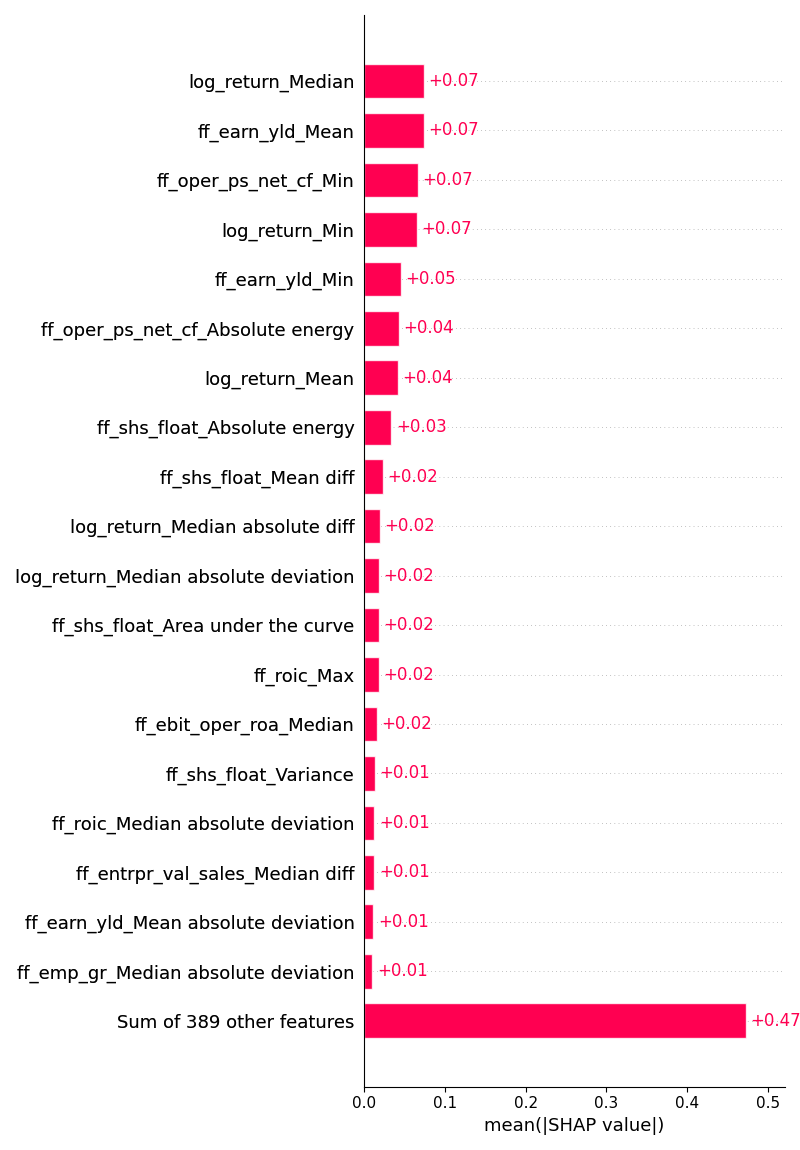
\includegraphics[width=\textwidth]{../Stock-Implosion-Prediction-FYP/pipelines/results_1yr/XGB_shap_bar.png} % Replace 'image_filename' with the name of your image file
    \caption{SHAP Absolute Values (XGBoost)}
    \label{fig:xgb_shap_if}
  \end{subfigure}
  \hfill
  \begin{subfigure}[b]{0.45\textwidth} % Adjust the width as needed
    \centering
    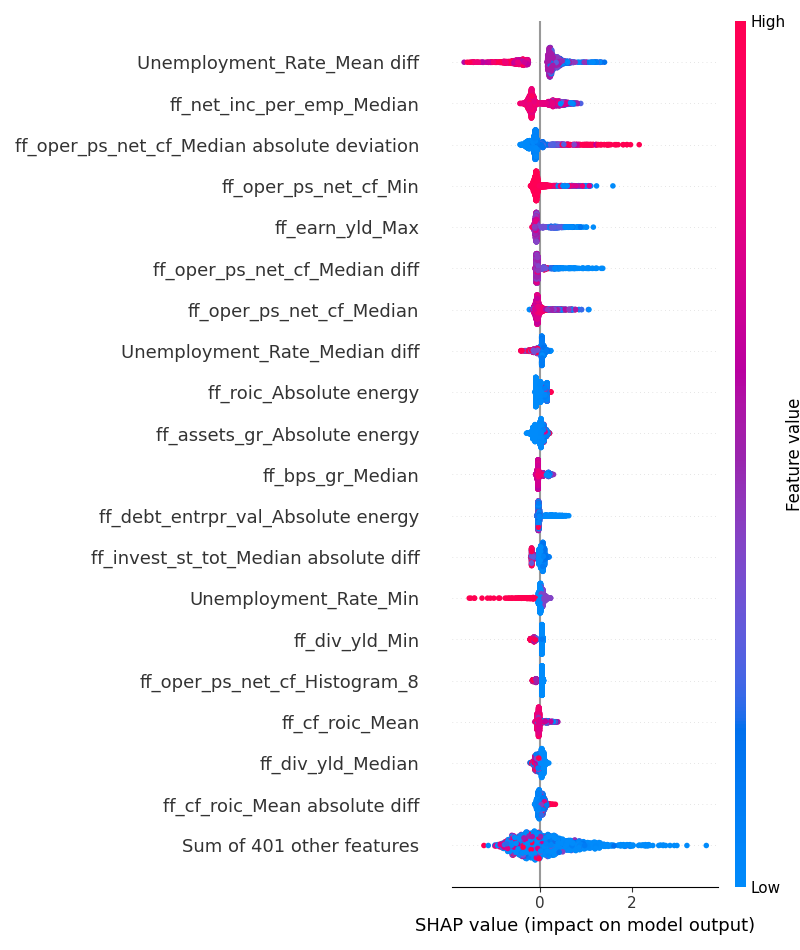
\includegraphics[width=\textwidth]{../Stock-Implosion-Prediction-FYP/pipelines/results_1yr/XGB_shap_beeswarm.png} % Replace 'image_filename' with the name of your image file
    \caption{SHAP Beeswarm (XGBoost)}
    \label{fig:xgb_shap_if_beeswarm}
  \end{subfigure}
  \caption{XGBoost SHAP Plots}
  \label{fig:shap_comparison}
\end{figure}



\section{Results (Approach 2 - 5-year Rolling Window)}

\subsection{Results}
The results for the 5-year rolling window experiment can be observed in Table \ref{tab:model_evaluation_all}.
\begin{table}[htbp]
  \centering
  \caption{Model Evaluation Results (Approach 2 - 5-year Rolling Window)}
  \label{tab:model_evaluation_all}
  \begin{adjustbox}{max width=\textwidth}
  \begin{tabular}{lcccccccccc}
    \toprule
    Model & Precision (0) & Precision (1) & Recall (0) & Recall (1) & F1 Score (0) & F1 Score (1) & MCC\\
    \midrule
    LR & 1.00 & 0.06 & 0.88 & 0.80 & 0.94 & 0.11 & 0.21  \\
    RF & 1.00 & 0.22 & 0.99 & 0.46 & 0.99 & 0.30 & 0.31  \\
    GBT & 1.00 & 0.08 & 0.92 & 0.79 & 0.96 & 0.15 & 0.24 \\
    XGB & 1.00 & 0.25 & 0.99 & 0.48 & 0.99 & 0.33 & 0.35 \\
    MLP & 1.00 & 0.14 & 0.97 & 0.50 & 0.98 & 0.22 & 0.26  \\
    \bottomrule
  \end{tabular}
  \end{adjustbox}
\end{table}The Logistic Regression model, despite its high recall, proves inferior to the others due to its low precision in the implosion class. It is clear that the model is not able to fit a linear relationship between the factors 
and risk of implosion. The MLP, somewhat surprisingly, suffers similar results. It is worth mentioning that due to the number of hyperparameters, the MLP is by far the most 
sensitive to hyperparameter tuning. Thus, such results suggest that the architecture found may not be the optimal one, and deeper models may be required. However, deeper models 
are prone to overfitting, so one must explore this option with caution. The GBT model also exhibits high recall and miniscule precision, conveying a failure to capture 
any significant underlying patterns in the data - it is likely that this is the result of the PySpark limitations on hyperparameter tuning. Since trees are restricted to a maximum 
depth of 30, it can become more challenging to achieve homogeneous groups. However, the PySpark Random Forest presents itself as a viable option for predicting implosions, achieving an MCC of 0.31 despite 
a perhaps lower than desirable precision. Finally, the XGBoost model achieves the highest MCC of 0.35 and the highest precision of 0.25, thus making it the strongest-performing 
model. Hence, XGBoost proves the most versatile option for predicting implosions - the stronger focus on recall aligns well with investor perspectives, yet the modest 
precision avoids a complete erasure of the portfolio. Despite this, there is still plenty of room for improvement - although the balance is correct, a more effective model would have higher scores in both categories.

\subsection{False Positives Analysis}
However, these results do not convey the full picture. Indeed, while the model seems to achieve more false positives than desired, it is crucial to remember that the model is classifying \textit{implosion years}. There are many cases 
where the model predicts Catastrophic Implosions too early. For these stocks, since the periods following after share similar characteristics, such as lower earnings yields and cash flows, these are also predicted to be implosion years. Hence,
in these cases, the model follows less in the lines of a crash prediction model and more in line with financial distress prediction. Linking back to the \textit{which} vs \textit{when} subproblems, the model is able to successfully 
detect implosions over a large proportion of stocks but, within each stock, finds it tougher to pinpoint the exact timing of the point of implosion. However, as noted previously, from an investor perspective solving the \textit{which} 
problem holds much more significance, still allowing for the elimination of stocks at risk of Catastrophic Implosion, despite ambiguity about timing. 

observing these false positives (Figure \ref{fig:not_detected_implosions}) suggests that 
many of these stocks do implode. 


The red regions in Figure \ref{fig:not_detected_implosions} reflects a predicted implosion year (year where the implosion occurs, not the exact point of implosion) that does not classify, under the study's interpretation, as a Catastrophic Implosion. Yet
many of these regions do consist of crashes/implosions that investors would very likely prefer to avoid. Thus, one may argue that the low precision is a limitation of the definition itself, and not the model. As noted in Chapter 3, the definition provides a starting point for 
modelling Catastrophic Implosions, but is by no means perfect.

% Similarly, one can view the false negatives predicted by the model 
% in Figure \ref{fig:missed_implosions}, reflecting implosions that were not captured (the green regions are implosion years). 


\subsection{Feature Importances}
Figure \ref{fig:xgb_5yr_feats} illustrates the Gini Importances for the XGBoost model. The bar plot displays high importance associated 
with the following features:
\begin{enumerate}
  \item Earnings Yield
  \item Cash Flow from Operations per Share
  \item Log Returns
  \item Dividend Yields
\end{enumerate}
Similar to Approach 1, SHAP values on the test set are also calculated to give a stronger idea of how these features impact model predictions.
\begin{figure}[h] 
  \centering
  \includegraphics[width=0.9\textwidth]{../Stock-Implosion-Prediction-FYP/pipelines/results_5yr/XGB_feature_importances.png} % Replace 'image_filename' with the name of your image file
  \caption{Approach 2 - 5-year Rolling Window - Feature Importances (XGBoost)}
  \label{fig:xgb_5yr_feats}
\end{figure}In Figure \ref{fig:xgb_5yr_feats} the absolute SHAP values and SHAP beeswarm plots are illustrated for XGBoost, the former providing another representation of the key drivers of the model, 
and the latter providing insights into the impact of each feature on predictions. Analysing Figure \ref{fig:comparison_shap_5yr} highlights how higher log returns, earning yields and cash flows from operations
are more likely to push the model to predict a non-implosion, and lower log returns (in particular, log return medians) steer the model in the implosion direction.

\begin{figure}[H] % 'h' specifies to place the figure here
  \centering
  \begin{subfigure}{0.45\textwidth} % Adjust width as needed (e.g., 0.5\textwidth for half the width)
      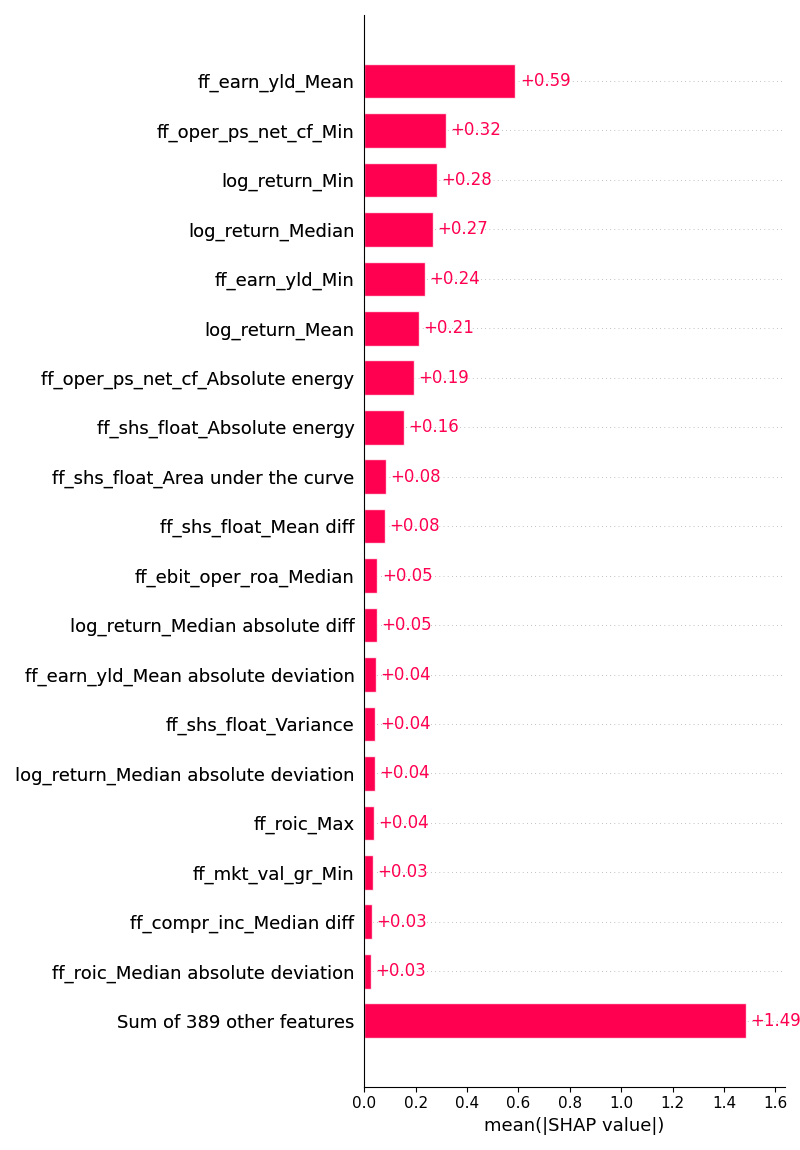
\includegraphics[width=\linewidth]{../Stock-Implosion-Prediction-FYP/pipelines/results_5yr/XGB_shap_bar_final.png} % Replace 'image_filename' with the name of your image file
      \caption{SHAP Absolute Values (XGBoost)}
      \label{fig:xgb_when_shap}
  \end{subfigure}
  \begin{subfigure}{0.45\textwidth} % Adjust width as needed (e.g., 0.5\textwidth for half the width)
      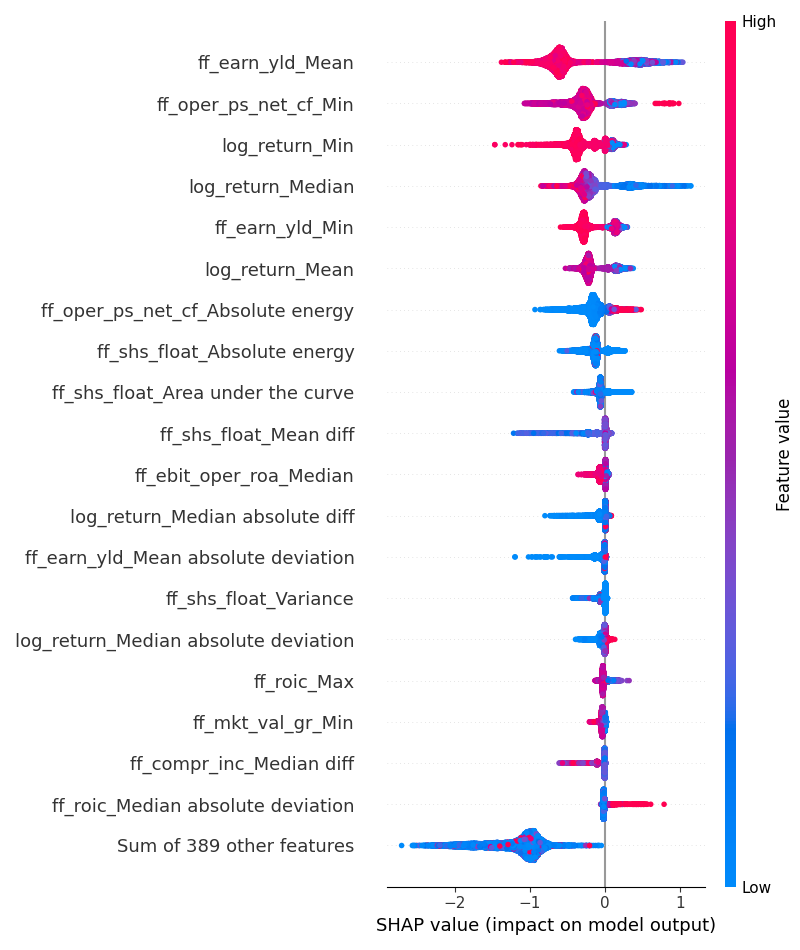
\includegraphics[width=\linewidth, height=9cm]{../Stock-Implosion-Prediction-FYP/pipelines/results_5yr/XGB_shap_beeswarm_final.png} % Replace 'image_filename' with the name of your image file
      \caption{SHAP Beeswarm (XGBoost)}
      \label{fig:xgb_when_shap_bee}
  \end{subfigure}
  \caption{Comparison of Feature Importances}
  \label{fig:comparison_shap_5yr}
\end{figure}These feature importances, while not enough to establish a causal dependence, provide a starting point for further investigation. For instance, looking closer at earnings yields, Figure \ref{fig:earn_yld_boxplot}
illustrates a significant difference in the distribution between the two classes, providing further evidence that imploded stocks indeed suffer from much lower earnings than those that do not implode. 
\begin{figure}[H] % 'h' specifies to place the figure here
  \centering
      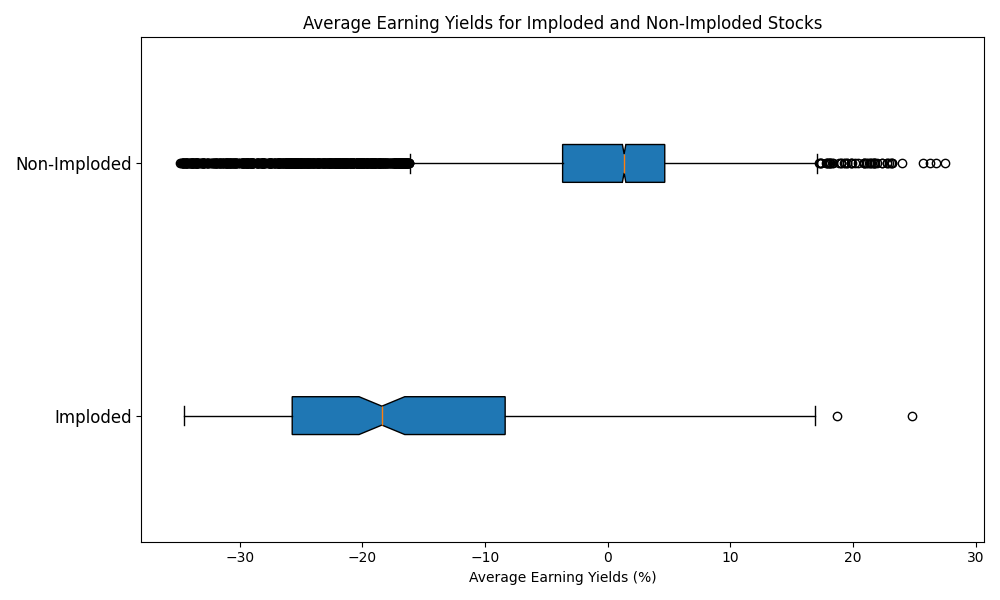
\includegraphics[width=0.6\linewidth]{../Stock-Implosion-Prediction-FYP/pipelines/results_5yr/earn_ylds_boxplot.png} % Replace 'image_filename' with the name of your image file
      \caption{Box Plot - Average Earnings Yields - Imploded vs Non-Imploded Stocks}
      \label{fig:earn_yld_boxplot}
  \caption{Earnings Yields}
  \label{fig:earn_ylds_plots}
\end{figure}Surprisingly, the industry variables do not seem to have a major impact on the model's splitting criterion. According to the model, variables such as earnings yields and cash flow 
overpower any potential correlations between Catastrophic Implosions and industry. Taking a look at Acorda Therapeutics, one of the pharmaceuticals companies discussed in the first chapter, 
the model predicts

\section{The Optimal Approach}
Having evaluated both Approach 1 and 2, it can be concluded that leveraging a 5-year rolling window successfully yields higher classification results across the board than a 1-year rolling window. Despite this, there are 
some important limitations of Approach 2 that Approach 1 does not suffer from. The requirement of a 5-year rolling window requires stocks that have at least 5 years worth of data. While this does not affect the class imbalance,
it does result in a smaller selection of stocks assessed in comparison to Approach 1. Furthermore, the additional steps of Boruta and TSFEL aggregation, while powerful, are very computationally expensive (one of the motivators
for using a yearly time series). Finally, while TSFEL proves powerful for feature extraction, the consequence is that it can be more challenging to decipher feature importances. For instance, while the average earnings yields 
of a corporate proves to have a profound effect on model predictions, looking at the average does not give any indication of where in the 5 year rolling window the specific change occurred. Nevertheless, the main objective of 
this study remains to detect as many implosions as possible before they occur, and to this extent Approach 2 is clearly superior.


% Having discussed the results generated from each methdology, what method is optimal for implosion prediction? Table \ref{tab:model_comparison} provides 
% a final summary of the advantages and disadvantages of each approach.
% \begin{table}[ht]
%   \centering
%   \caption{Advantages and Disadvantages of Two Methodologies}
%   \label{tab:model_comparison}
%   \begin{tabular}{p{0.25\linewidth}p{0.4\linewidth}p{0.4\linewidth}}
%   \toprule
%   \textbf{Aspect} & \textbf{1-year Rolling Window} & \textbf{5-year Rolling Window} \\
%   \midrule
%   \textbf{Advantages} & 
%   \begin{itemize}
%       \item Covers a larger number of stocks and implosions over a wider timeframe.
%       \item Requires less pre-processing.
%       \item Easier interpretation.
%   \end{itemize}
%   & 
%   \begin{itemize}
%       \item Each sample is assessed with five years of historical data instead of just one year.
%       \item Model results are stronger.
%   \end{itemize} \\
%   \midrule
%   \textbf{Disadvantages} & 
%   \begin{itemize}
%       \item Smaller, 1-year rolling window.
%       \item Weaker results.
%   \end{itemize}
%   & 
%   \begin{itemize}
%       \item TSFEL computationally expensive.
%       \item Can be more challenging to interpret due to aggregations.
%       \item Only covers stocks with at least 5 years of historical data.
%   \end{itemize} \\
%   \bottomrule
%   \end{tabular}
% \end{table}As highlighted in Table \ref{tab:model_comparison} and the prior Results sections, Approach 2 excels over Approach 1 in performance - utilizing 
% a 5-year rolling window demonstrates a substantial increase in performance, with the best model of Approach 2 (XGB) achieving an MCC of 0.35, greater than 
% the best of Approach 1 (GBT - 0.22). Despite this, there are some important limitations to be discussed about Approach 2. The use of a 5-year rolling 
% window means that only stocks with 5 years worth of data can be assessed. While this does not significantly impact the class imbalance (it is slightly lower than 
% that of Approach 1), it does result in a reduction of stocks assessed overall. In addition, this also means the model is trained on implosions that occur from 2006 onwards,
% ignoring the Dot-Com bubble where significant implosions did occur (Figure \ref{fig:implosions_year}). Since Approach 1 only requires one year worth of data to be available, 
% the model is assessed over a wider universe and timeframe. Another drawback of Approach 2 comes with interpretability - while the aggregations may enhance model performance,
% interpreting them over a 5-year window can be more challenging. For instance, it is difficult to pinpoint when a change in earnings/assets occurred that led to the prediction 
% of an implosion, as the entire 5 years is represented by the single, aggregated value. For Approach 1 it is much simpler to understand whether, for a given implosion, earnings/assets 
% ratio was higher or lower the year prior.\\\\Nevertheless, the limitations of Approach 2 do not overpower its value from a practical, performance-based perspective. Achieving higher MCC 
% scores across all models tested, it remains the superior approach for capturing implosions both more frequently and with a higher consistency of being correct. Thus, one may 
% conclude that the incorporation of longer-term historical data is more likely to provide stronger results than a shorter-term window, provided the feature space is suitably engineered.

\section{Summary}
This chapter commenced with an overview of the strategies leveraged for model improvement and effective evaluation. Class weighting was applied to penalize the misclassification 
of implosions during training, and Bayesian Optimization for hyperparameter tuning was applied for efficient exploration into selecting the best model architectures. Results demonstrate that Approach 2
was more successful than Approach 1, signifying the value of longer-term historical data as opposed to shorter-term for predicting Catastrophic Implosions. An XGBoost model was developed, achieveing
an MCC of 0.35, recall of 0.61 and precision of 0.20. Despite the lower precision, it was illustrated that many of the false positives produced by the model were actually the result of a mismatch in timing, or 
an implosion that did not quite fit the proposed definition. It was highlighted that the definition for a Catastrophic Implosion proposed in this study is by no means perfect, and was used 
as a starting point for further investigations into related metrics for quantifying corporate failure. The use of feature importance techniques suggested earnings yields, earnings/assets ratios and 
operating cash flow play significant roles in model predictions, prompting their inclusion in future definitions and models.

\chapter{Conclusions and Future Work}
\textit{The investigation concludes by re-stating the objectives and highlighting whether these have been achieved. There is also discussion regarding the limitations behind the investigation and areas
for improvement. Finally, the investigation points directions for next steps in the field.}

\section{Achievements}
The investigation aimed to solve the following problem:\\\\\textit{Can corporate fundamentals be used to predict Catastrophic Implosions effectively?}\\\\Based on empirical results, there 
is evidence that corporate fundamentals can be leveraged to forecast implosions. The gradient boosting model from Approach 1 - Imploding Stock Prediction attains an overall 
MCC score of 0.56, indicating a strong albeit not perfect ability to distinguish imploding stocks from healthy stocks. Its precision of 0.78 conveys 
reliability - when the model does forecast an implosion, it is likely to be correct. Potential strategies for improving recall may include experimenting over 
a larger dataset, more timeframes and leveraging deeper machine learning models. The initial exploratory analysis highlights the impact of market value (with majority 
of implosions occurring over smaller-cap stocks) and industry (the Pharmaceuticals industry consistently suffering). Upon prediction, the following features
\begin{enumerate}
  \item Earnings/Assets Ratio
  \item Net income
  \item Cash Flow from Operations per Share
\end{enumerate}
were found to drive implosions cross-sectionally over the 10,000 stocks universe. These features can be incorporated into future prediction models and even be monitored by portfolio managers for warning signals. Note that Earnings/Assets 
Ratio is the \(b\) term in the Altman Z-score (equation \ref{eq:z-score}), conveying alignment with prior prediction models.
Furthermore, the stronger results attained from Approach 1 
compared to Approach 2 suggest that the historical characteristics of stocks remains crucial for predicting implosions - it is much tougher to predict implosions based 
on current year fundamentals only. 

\subsection{Research Objectives}
A summary of each research objective and how it was achieved is given below:

\subsubsection{Define 'Catastrophic Stock Implosion'}
The investigation explores various metrics for defining catastrophic stock implosions. The framework for implosions was defined in two parts: first identifying a significant deviation 
in price, followed by an increased period of low growth. The deviation was quantified by observing a 80\% fall in cumulative returns, and the period following was 
monitored to ensure the cumulative return remained below 20\% from the price at fall. 

\subsubsection{Analyse and Select Suitable Features}
The investigation utilized several techniques for feature selection and extraction, including the innovative use of TSFEL to derive over 900 
additional statistically and temporally aggregated features. Such feature engineering techniques proved to have a tremendous effect on model performance. 

\subsubsection{Develop Suitable Methodology}
The investigation explores two realms of implosion classification. The first approach seeks to label stocks as \textit{imploding} based on their current history, 
while the second approach aims to understand what factors cause an implosion in a given year.

\subsubsection{Implement Model Effectively}
To achieve strong, effective results several tuning and adjusting strategies were designed, including the use of class weighting, bayesian hyperparameter optimization, feature 
extraction and feature elimination. A range of models varying in complexity were experimented with, ranging from Logistic Regression to Neural Networks. 

\subsubsection{Derive Key Factors Driving Implosions}
By leveraging Gini Importance and Shapley values, the key factors driving the models were analysed. Results suggest the use of
earnings, assets, cash flow and macroeconomic variables as potentially powerful indicators that should be monitored by investors and factored in to other models for 
implosion prediction and related tasks. 

\section{Limitations}
A key limitation was the use of yearly data throughout both methodologies. The choice for yearly as opposed to quarterly data was made for several reasons. The primary 
advantage is the reduction in class imbalance - changing the frequency to quarterly would widen the imbalance gap between each class even further, since only one specific quarter 
would be labelled as imploded, not the whole year. This would also result in higher computational costs. Nevertheless, the usage of quarterly or even weekly data may allow for 
more precision, but a great deal of additional research may be necessary to assess the best methodology and model to use. These ideas are discussed further in the following section.

\section{Future Work}
The investigation opens up possible directions for future work. Neural networks have shown great promise in the fields of stock market forecasting and bankruptcy prediction. While 
the investigation experimented with basic architectures such as MLPs, complex, temporal models such as RNNs and LSTMs remain to be investigated. Rather than investigate every possible model,
the investigation focused on formulating the underlying strategies with which these models would be deployed. Furthermore, there are some limitations to using these more complex models. First 
is the cost to interpretability - it is much more challenging to identify the driving features behind MLPs, RNNs and LSTMs as compared to Decision Trees and Random Forests due to their 
sequential nature and model complexity. In addition, such models require significant preprocessing of data, generally requiring fixed length input sequences which does not fit 
the current domain, since stocks have different time frames. Nevertheless, RNNs and LSTMs have shown great performance in the field of 
time series forecasting due to their ability to capture temporal patterns. For those mainly interested in accuracy, it is likely that such models can offer on par if not better 
results if configured correctly.\\\\Another potential direction of research is to experiment with Unsupervised Learning. While there was some investigation into the use of Isolation Forest 
to detect implosions(modelling implosions as anomalies across the stock universe), a deeper dive into models such as Autoencoders may lead to more promising results. The benefit 
of utilizing an unsupervised approach is that the requirement for labelling is not needed - indeed, as highlighted in Chapter 3, defining a catastrophic stock implosion quantitatively 
is challenging, and the false positives obtained by the XGBoost model in Figure \ref{fig:wrong_implosions_if} suggest limitations to the approach used in the investigation. Hence, an unsupervised model, if calibrated correctly, could be used to detect implosions as anomalies.
However, the main hurdle is ensuring that implosions are the only type of anomalies that are detected by the model - for e.g., it may be difficult for an unsupervised algorithm 
to distinguish between an upward spike and a downward spike, as one could argue that they are both 'anomalies'.\\\\Finally, as highlighted in Chapter 5, the driving features 
can be utilized to redefine and improve the definition of a catastrophic stock implosion and related 
events such as stock crashes and financial distress - as highlighted in Chapter 2 there remains inconsistency across the definitions used in related literature. Beyond price and market value, 
the findings in this investigation suggest a negative correlation between earnings/assets ratios and cash flow against implosion risk. The impact of macroeconomic variables such as Unemployment Rate is also apparent, with 
more implosions occurring during periods of economic distress. Hence, a multi-criteria definition can be built according to these factors, where an implosion would be detected based on one (or potentially all) of these variables falling past a particular threshold. 
The investigation leaves the door open for continued innovations to demystify the nature of catastrophic stock implosions and bolster risk mitigation strategies for portfolio management.


% \begin{thebibliography}{HHM99}


% \bibitem[Pri70]{PriorNOP70}  %%only an example
% A.~Prior.
% \newblock The notion of the present.
% \newblock {\em Studium Generale}, 23:  245--248, 1970.


% \bibitem[Rey97]{Rey:D}
% M.~Reynolds.
% \newblock A decidable temporal logic of parallelism.
% \newblock {\em Notre Dame Journal of Formal Logic}, 38(3):  419--436,
%   1997.

% \end{thebibliography}
\bibliographystyle{apalike} 
\bibliography{bib}
 % Choose a bibliography style



\newpage
\appendix
\renewcommand{\thefigure}{A\arabic{figure}}
\renewcommand{\thetable}{A\arabic{table}} % Redefine figure numbering to include the letter A for appendix
\chapter*{Appendix A} 


\section*{Code for Labelling Implosions}


\begin{algorithm}
  \caption{Finding Implosions via Price Metric}
  \label{alg:find_implosions}
  \begin{algorithmic}[1]
      \Procedure{FindImplosionPrice}{$df1$}
    \State $imp\_dates \gets []$
    \State $i \gets 26$
    \While{$i < \text{length}(df1)$}
        \State $current\_date \gets df1.loc[i, 'date']$
        \State $current\_price \gets df1.loc[i, 'adj\_price']$
        \If{$df1.loc[i, 'cum\_return'] < price\_drop\_thresh$}
            \State $j \gets i$
            \State $start\_price \gets current\_price$
            \State $j \gets j + 1$
            \State $imp\_period \gets 0$
            \While{$j < \text{length}(df1)$ and $\frac{(df1.loc[j, 'adj\_price'] - start\_price)}{start\_price} \leq increase\_thresh$}
                \State $imp\_period \gets imp\_period + 1$
                \State $j \gets j + 1$
            \EndWhile
            \If{$imp\_period > period\_thresh$}
                \State $imp\_dates$.append($(current\_date, df1.loc[i + imp\_period, 'date']))$
            \EndIf
            \State $i \gets i + imp\_period$
        \EndIf
        \State $i \gets i + 1$
    \EndWhile
    \If{$\text{length}(imp\_dates) > 0$}
        \State $df1.loc[df1['fsym\_id'] == fsym\_id, 'Implosion\_Start\_Date'] \gets imp\_dates[0][0]$
        \State $df1.loc[df1['fsym\_id'] == fsym\_id, 'Implosion\_End\_Date'] \gets imp\_dates[0][1]$
    \EndIf
    \State \textbf{return} $df1$
\EndProcedure
  \end{algorithmic}
  \end{algorithm}

\section*{Grid Search Results for Catastrophic Implosion Definition}
\begin{table}[htbp]
  \centering
  \small
  \caption{Grid Search Results}
  \label{tab:data_description}
  \begin{tabularx}{\textwidth}{|p{3cm}|p{3cm}|p{3cm}|p{4cm}|}
  \hline
  \textbf{price\_drop\_thresh} & \textbf{min\_impl\_period} & \textbf{impl\_thresh}  & \textbf{number of implosions} \\ 
  \hline
  -0.6 & 78  & \(-0.2\) & 1056 \\
  -0.6 & 78  & \(+0.0\) & 2120 \\
  -0.6 & 78  & \(+0.2\) & 2355 \\
  -0.6 & 104 & \(-0.2\) & 819 \\
  -0.6 & 104 & \(+0.0\) & 1647 \\
  -0.6 & 104 & \(+0.2\) & 1888 \\
  -0.7 & 78  & \(-0.2\) & 896 \\
  -0.7 & 78  & \(+0.0\) & 1718 \\
  -0.7 & 78  & \(+0.2\) & 1924 \\
  -0.7 & 104 & \(-0.2\) & 691 \\
  -0.7 & 104 & \(+0.0\) & 1336 \\
  -0.7 & 104 & \(+0.2\) & 1506 \\
  -0.8 & 78  & \(-0.2\) & 711 \\
  -0.8 & 78  & \(+0.0\) & 1283 \\
  -0.8 & 78  & \(+0.2\) & 1421 \\
  -0.8 & 104 & \(-0.2\) & 563 \\
  -0.8 & 104 & \(+0.0\) & 1024 \\
  -0.8 & 104 & \(+0.2\) & 1133 \\ 
  \hline
  \end{tabularx}
\end{table}





% \begin{figure}[h] % 'h' specifies to place the figure here
%   \centering
%   \begin{subfigure}{0.4\textwidth}
%     \centering
%     \includegraphics[width=\linewidth]{../Stock-Implosion-Prediction-FYP/all_by_industry_pie.png} % Replace 'image_filename' with the name of your image file
%     \caption{Stocks By Industry}
%     \label{fig:industry_all}
%   \end{subfigure}
%   \begin{subfigure}{0.4\textwidth}
%     \centering
%     \includegraphics[width=\linewidth]{../Stock-Implosion-Prediction-FYP/all_by_industry_implosions_pie.png} % Replace 'image_filename' with the name of your image file
%     \caption{Implosions By Industry}
%     \label{fig:industry_implosions_pie}
%   \end{subfigure}
%   \caption{Comparison of Stocks and Implosions By Industry}
%   \label{fig:industry_comparison}
% \end{figure}

\appendix
\renewcommand{\thefigure}{B\arabic{figure}} % Redefine figure numbering to include the letter A for appendix
\chapter*{Appendix B} 

% \section*{Sample Implosions - Pharmaceuticals Industry}
% \begin{figure}[H] % 'h' specifies to place the figure here
%   \centering
%   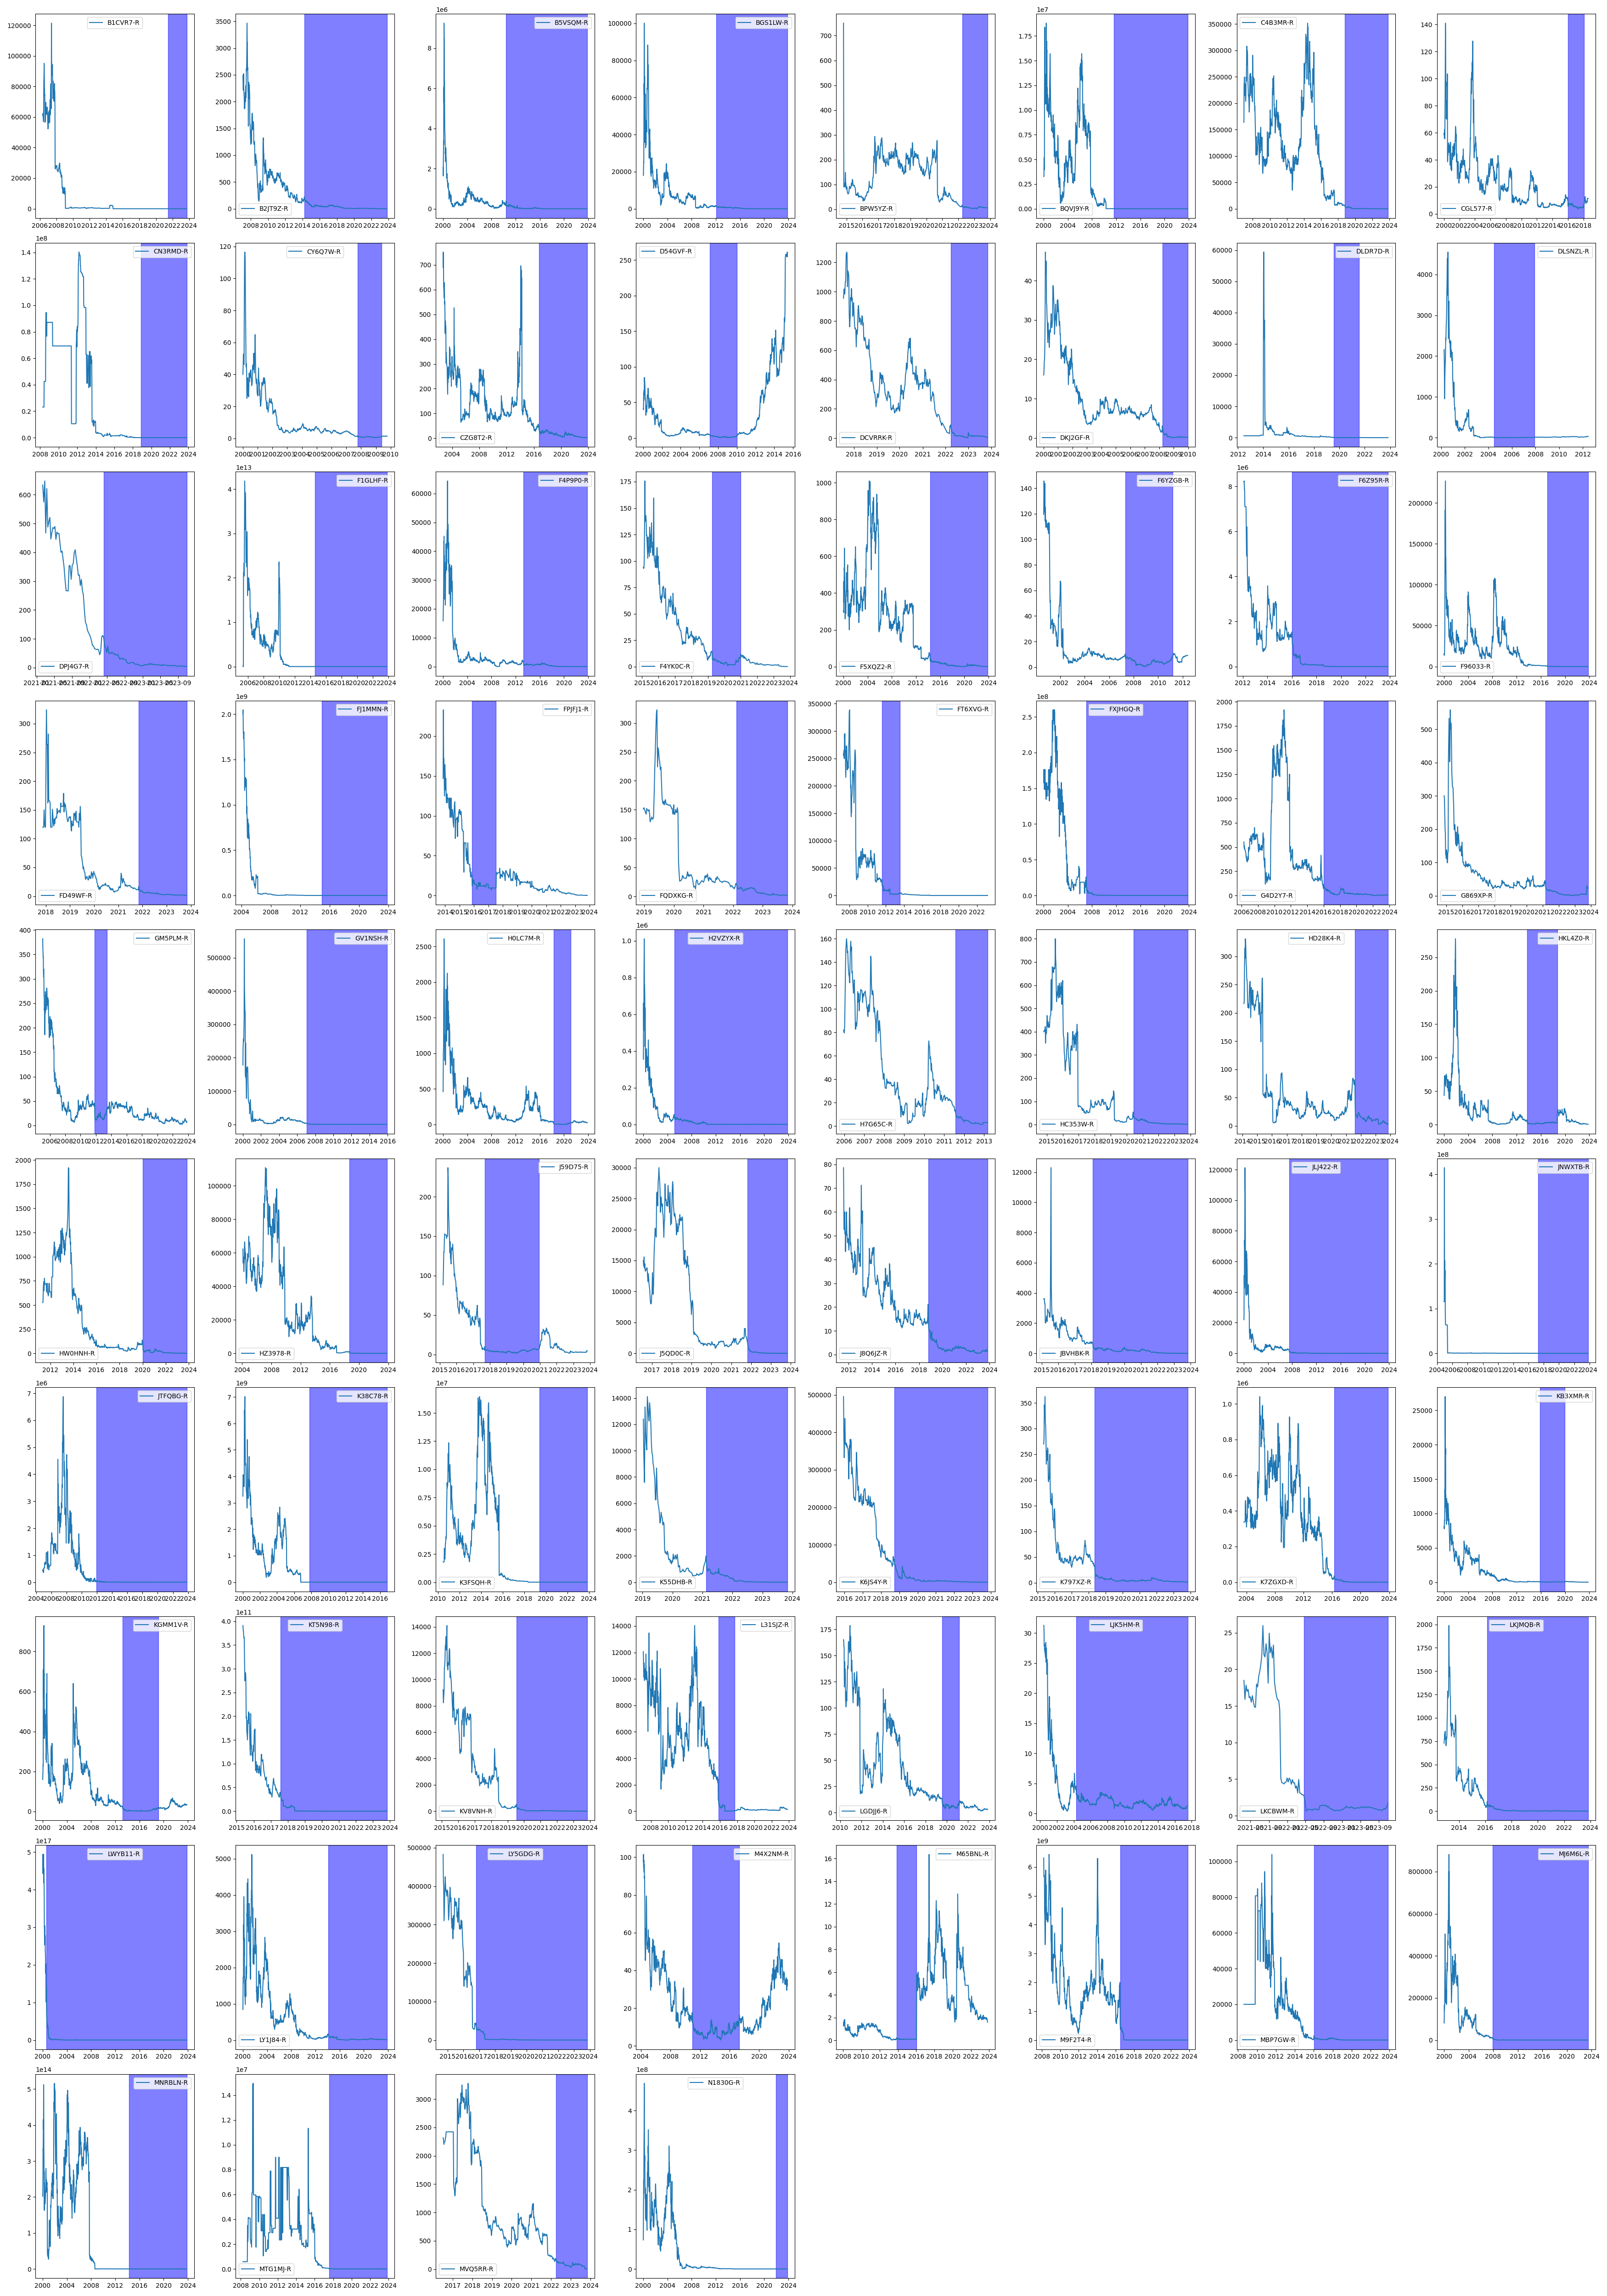
\includegraphics[width=1\textwidth]{../Stock-Implosion-Prediction-FYP/pharmaceuticals_implosions.png} % Replace 'image_filename' with the name of your image file
%   \caption{Sample of Implosions (Pharmaceuticals Industry)}
%   \label{fig:pharm_implosions}
% \end{figure}

\begin{figure}[h]
  \centering
  \includegraphics[width=1\textwidth]{eg_dd_doesnt_detect.png} % Replace 'image_filename' with the name of your image file
  \caption{Catastrophic Implosion (Gradual Decrease)}
  \label{fig:cum_ret_dd_scr}
  \medskip % Add some vertical space
  
  \parbox{\textwidth}{\footnotesize
  A comparison between using cumulative returns, drawdowns and Crash Risk for implosion identification. The stock 
  is an example of one that does not suffer a sudden drop, but rather a slower, more gradual fall. The highlighted region 
  reflects the implosion identified according to the criteria (no region means the stock did not implode according to the method).
  }
\end{figure}

\begin{figure}[h]
  \centering
  \includegraphics[width=1\textwidth]{cum_ret_sharp_eg.png} % Replace 'image_filename' with the name of your image file
  \caption{Catastrophic Implosion (Sharp Drop)}
  \label{fig:cum_ret_sharp}
  \medskip % Add some vertical space
  
  \parbox{\textwidth}{\footnotesize
  A comparison between using cumulative returns, drawdowns and Crash Risk for implosion identification. The stock is an example of 
  one that suffers a very sudden, sharp drop in price. The highlighted regions reflect the implosion according to each method's criteria
  (no region means the stock did not implode according to the method).
  }
\end{figure}

\section*{XGBoost (Additional Results)}

\begin{figure}[h] % 'h' specifies to place the figure here
  \centering
  \includegraphics[width=0.9\textwidth]{xgb_roc.png} % Replace 'image_filename' with the name of your image file
  \caption{XGBoost ROC}
  \label{fig:roc}
\end{figure}


\begin{figure}[h] % 'h' specifies to place the figure here
  \centering
  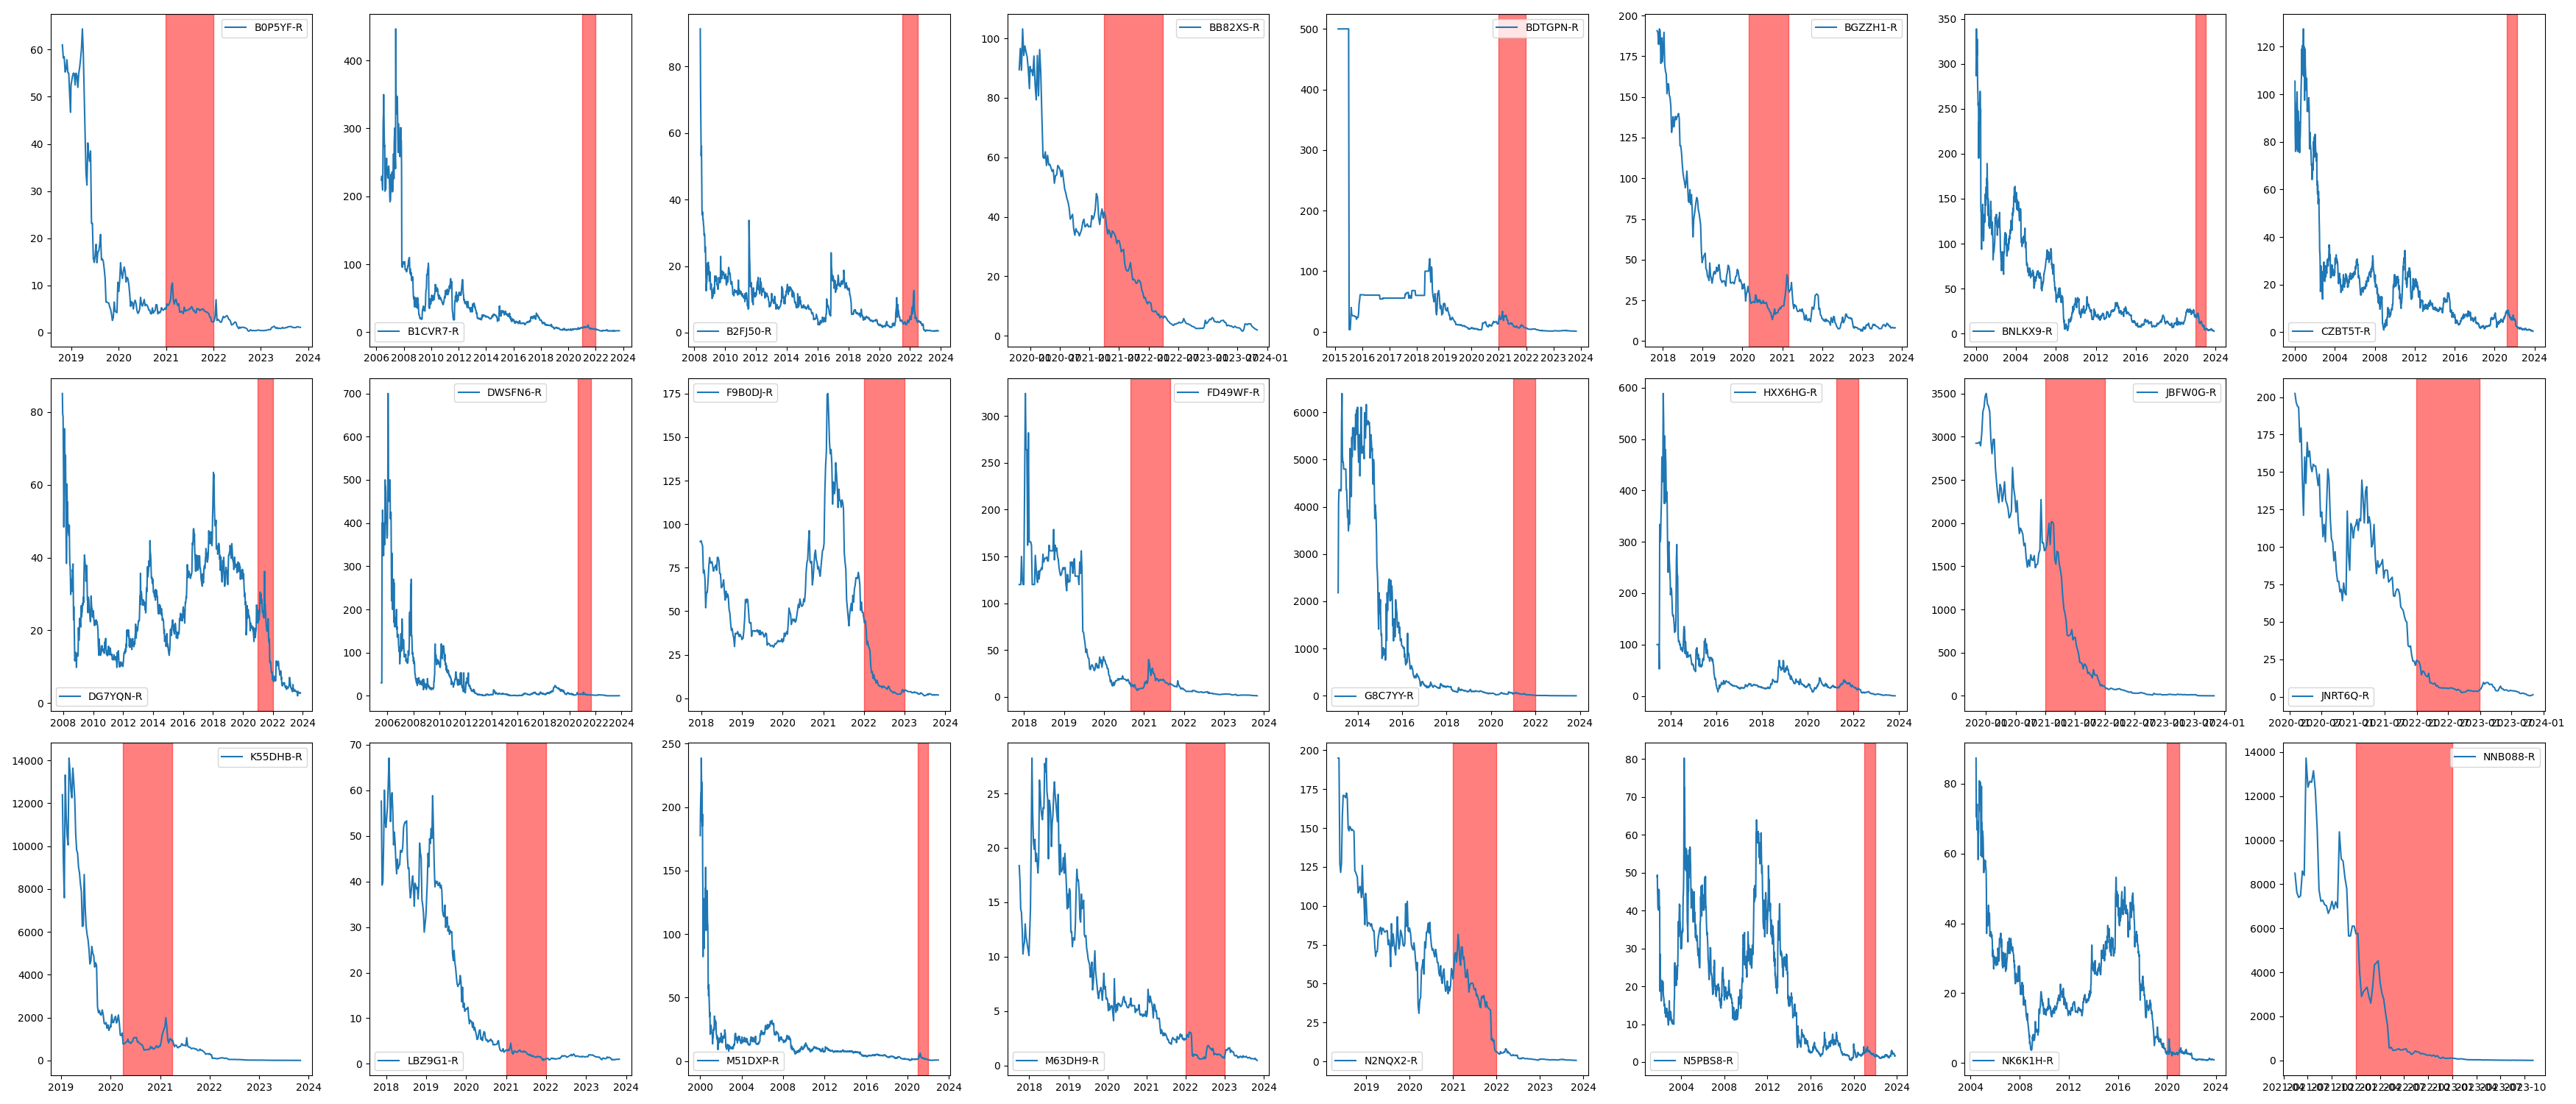
\includegraphics[width=0.9\textwidth]{../Stock-Implosion-Prediction-FYP/pipelines/results_5yr/incorrect_implosions_detected_by_model.png} % Replace 'image_filename' with the name of your image file
  \caption{Sample of False Positives - XGBoost - Approach 2- (5-year Rolling Window)}
  \label{fig:not_detected_implosions}
\end{figure}

\begin{figure}[h] % 'h' specifies to place the figure here
  \centering
  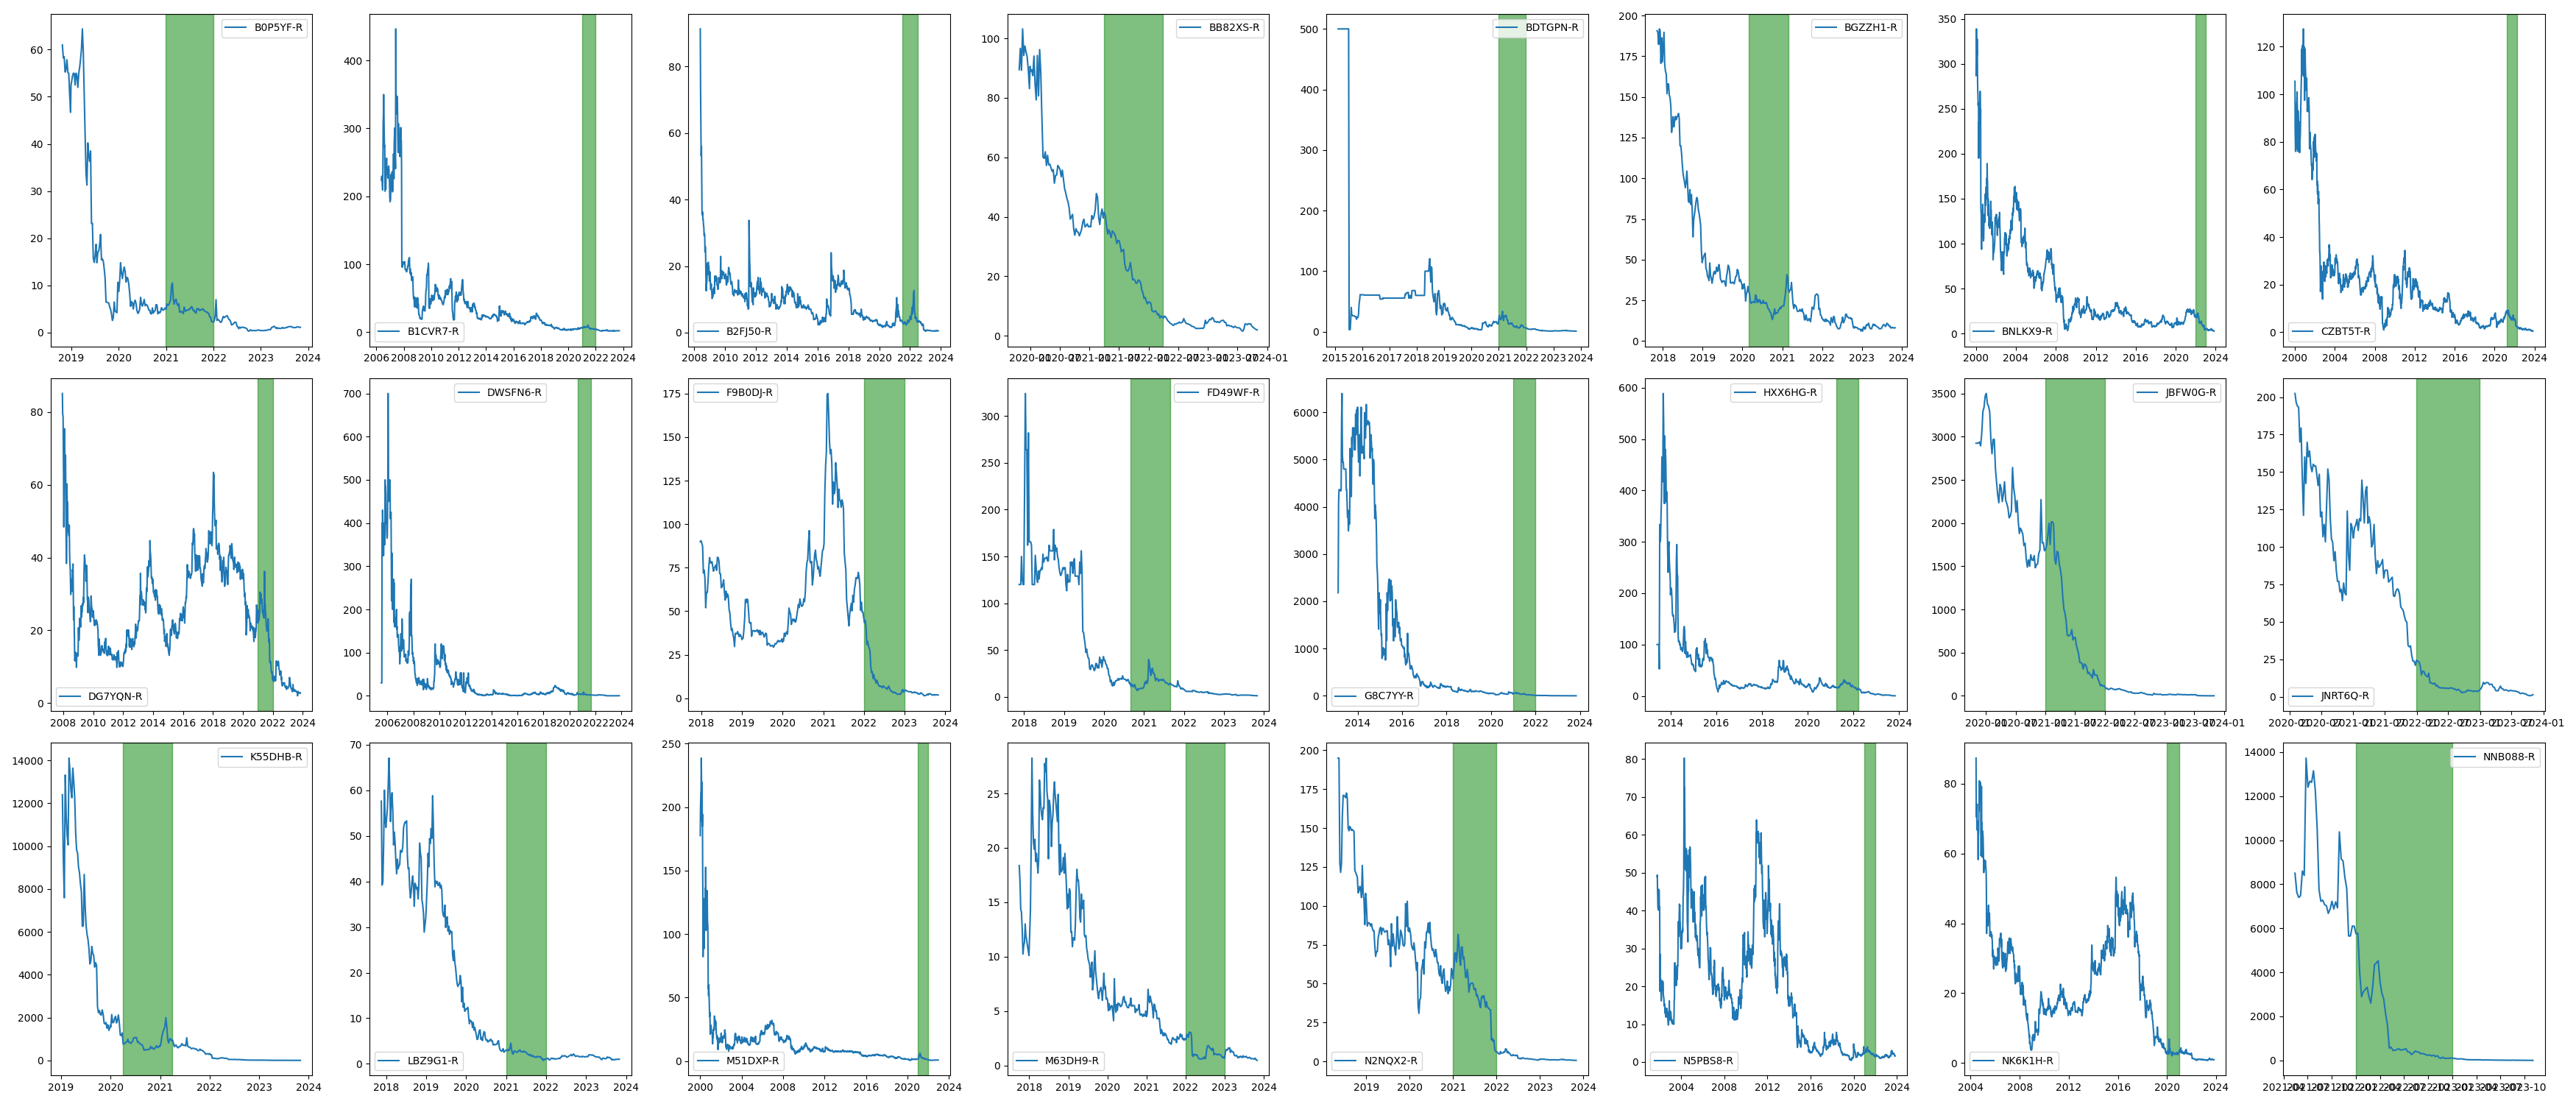
\includegraphics[width=0.9\textwidth]{../Stock-Implosion-Prediction-FYP/pipelines/results_5yr/missed_implosions.png} % Replace 'image_filename' with the name of your image file
  \caption{Sample of False Negatives - XGBoost - Approach 2- (5-year Rolling Window)}
  \label{fig:missed_implosions}
\end{figure}

% \begin{figure}[h] % 'h' specifies to place the figure here
%   \centering
%   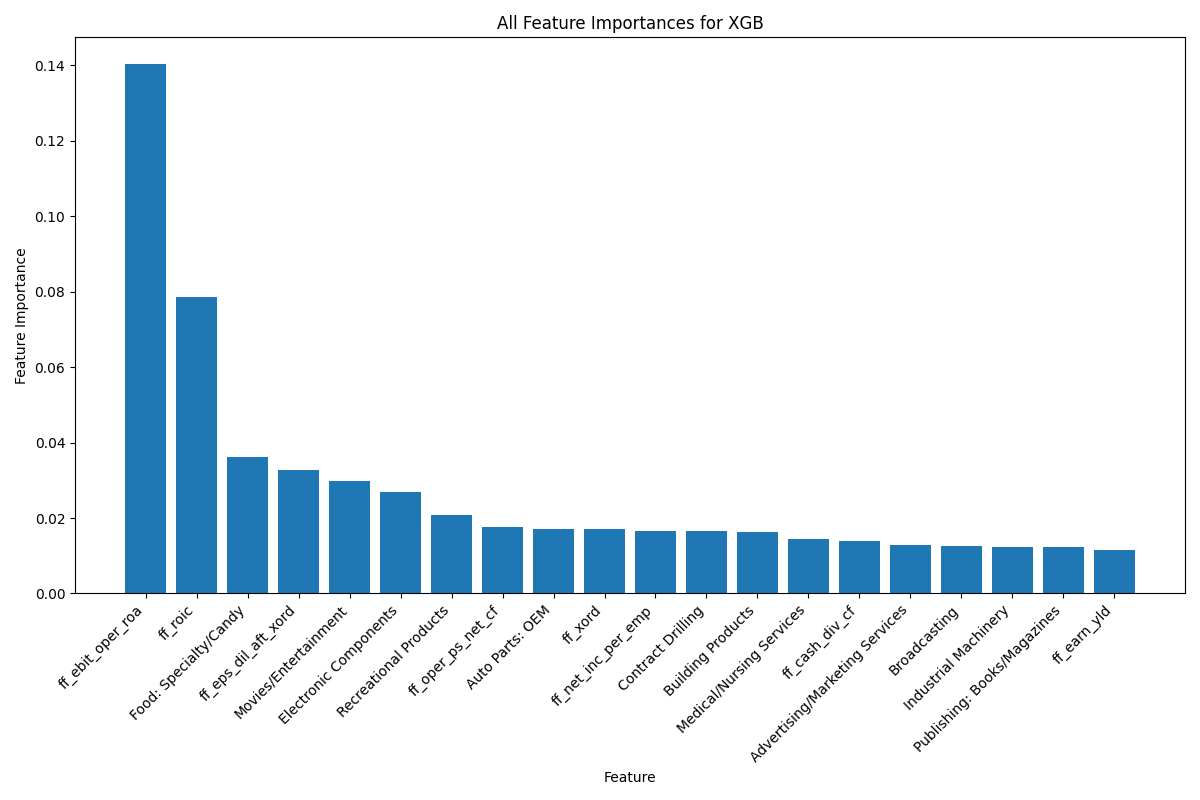
\includegraphics[width=0.9\textwidth]{../Stock-Implosion-Prediction-FYP/pipelines/results_when/XGB_all_feature_importances.png} % Replace 'image_filename' with the name of your image file
%   \caption{Approach 2 - Implosion Year Prediction - All Feature Importances (XGBoost)}
%   \label{fig:all_importances_when}
% \end{figure}

\end{document}